%% =====================================================================
%% REBEP -- Revista Brasileira de Estudos de Populacao
%% Submission source-of-truth for:
%%   "Multidimensional Racial Residential Segregation across Brazilian
%%    Cities: A Nationwide Assessment with 2022 Census Data"
%%
%% REBEP accepts Word (.doc/.docx) manuscripts ONLY -- it has no LaTeX
%% class. This file is the clean, versioned source; the author exports
%% it to Word (double-spaced, Arial or Times New Roman 12 pt) before
%% uploading. See SUBMISSION.md for the full checklist.
%%
%% Compile from draft/rebep/ :  pdflatex -> bibtex -> pdflatex x2
%%
%% Anonymisation: REBEP requires a fully anonymised manuscript (no author
%% identification anywhere, including PDF metadata). Toggle below.
%% =====================================================================

\newif\ifanon
\anontrue   % \anontrue  -> anonymised version for peer review (upload this)
            % \anonfalse -> identified version (keep for the camera-ready)

\documentclass[12pt,a4paper]{article}

%% Packages
\usepackage[utf8]{inputenc}
\usepackage[T1]{fontenc}
\usepackage{lmodern}
\usepackage{graphicx}
\usepackage{amsmath,amssymb}
\usepackage{booktabs}
\usepackage[round]{natbib}   % round brackets -> (Author, year), close to ABNT author-date
\usepackage{geometry}
\usepackage{setspace}
\usepackage{hyperref}
\usepackage{caption}
\usepackage{subcaption}
\usepackage{float}

\geometry{margin=2.5cm}
\onehalfspacing
\graphicspath{{../../figures/}}

\ifanon
  \hypersetup{pdfauthor={},pdftitle={}}
\fi

%% Title and Author
\title{Multidimensional Racial Residential Segregation across Brazilian Cities:\\
A Nationwide Assessment with 2022 Census Data}

\ifanon
  \author{}
  \date{}
\else
  \author{
  Renan Xavier Cortes\\
  Department of Statistics\\
  Federal University of Rio Grande do Sul\\
  Porto Alegre, Brazil\\
  \texttt{renan.cortes@ufrgs.br}
  }
  \date{\today}
\fi

\begin{document}

\maketitle

%% ---------------------------------------------------------------------
%% REBEP requires title, abstract and keywords in Portuguese, English AND
%% Spanish (abstract ~200 words each; up to 5 keywords from a standard
%% thesaurus -- IBICT/UNESCO/ERIC). Only the English block is filled here;
%% the Portuguese and Spanish versions are produced in Task 27 and must be
%% pasted below before submission.
%% ---------------------------------------------------------------------

\begin{abstract}
We provide a nationwide, multidimensional description of racial residential segregation in Brazilian cities. Using 2022 Census tract data, and the combined \emph{preta} and \emph{parda} population against the total population, we study the 319 municipalities above 100{,}000 inhabitants. For each we compute nine segregation indices spanning the five dimensions of Massey and Denton --- evenness, exposure, concentration, centralization and clustering --- with the PySAL segregation module, by point estimation without inference. Evenness segregation is moderate, with a median dissimilarity index near 0.20, and concentrated in the South and Southeast, confirming and extending earlier nationwide work on 2010 data. The four evenness indices are near-redundant (pairwise rank correlations of at least 0.92), but the other dimensions are not: the exposure dimension gives the opposite regional ranking, being highest in the North and Northeast, and this is compositional, as isolation tracks the local size of the minority population. The identity of the most segregated city depends entirely on the dimension chosen, the dissimilarity and isolation rankings correlating at a Kendall's $\tau$ of about $-0.26$. Two to three independent axes of variation underlie the indices. Characterising Brazilian racial segregation through the dissimilarity index alone is insufficient; a multidimensional, spatially explicit approach is needed.
\end{abstract}

\noindent\textbf{Keywords:} Residential segregation; Race; Brazil; 2022 Census; Spatial demography

%% --- PORTUGUESE / SPANISH front matter (REBEP requires all three) ---
%% Title, abstract (~200 words) and keywords only. The body stays in
%% English; REBEP handles body translation after acceptance. The
%% Portuguese and Spanish abstracts below were drafted by translation
%% and should be proof-read by a native speaker before submission.

\vspace{1.5em}
\begin{center}\textbf{\large T\'itulo e resumo em portugu\^es}\end{center}

\noindent\textbf{Segrega\c{c}\~ao residencial racial multidimensional nas cidades
brasileiras: uma an\'alise nacional com dados do Censo 2022}

\medskip
\noindent\textbf{Resumo.} Apresentamos uma descri\c{c}\~ao nacional e
multidimensional da segrega\c{c}\~ao residencial racial nas cidades brasileiras.
Com dados dos setores censit\'arios do Censo 2022, e a popula\c{c}\~ao
\emph{preta} e \emph{parda} somada frente \`a popula\c{c}\~ao total, estudamos os
319 munic\'ipios com mais de 100 mil habitantes. Para cada um calculamos nove
\'indices que abrangem as cinco dimens\~oes de Massey e Denton --- uniformidade,
exposi\c{c}\~ao, concentra\c{c}\~ao, centraliza\c{c}\~ao e agrupamento --- com o
m\'odulo \texttt{segregation} do PySAL, por estima\c{c}\~ao pontual, sem
infer\^encia. A segrega\c{c}\~ao de uniformidade \'e moderada, com \'indice de
dissimilaridade mediano pr\'oximo de 0,20, e concentra-se no Sul e no Sudeste,
confirmando e ampliando an\'alises nacionais anteriores com dados de 2010. Os
quatro \'indices de uniformidade s\~ao quase redundantes (correla\c{c}\~oes de
postos de pelo menos 0,92), mas as demais dimens\~oes n\~ao: a exposi\c{c}\~ao
inverte o ordenamento regional, sendo mais alta no Norte e no Nordeste, o que
\'e composicional, pois o isolamento acompanha o tamanho local da popula\c{c}\~ao
minorit\'aria. A cidade mais segregada depende inteiramente da dimens\~ao
escolhida: os ordenamentos por dissimilaridade e por isolamento correlacionam-se
a um $\tau$ de Kendall de cerca de $-0{,}26$. Duas a tr\^es dimens\~oes
independentes de varia\c{c}\~ao subjazem aos \'indices. Caracterizar a
segrega\c{c}\~ao racial brasileira apenas pela dissimilaridade \'e insuficiente;
\'e necess\'aria uma abordagem multidimensional e espacialmente expl\'icita.

\medskip
\noindent\textbf{Palavras-chave:} Segrega\c{c}\~ao residencial; Ra\c{c}a; Brasil;
Censo 2022; Demografia espacial

\vspace{1.5em}
\begin{center}\textbf{\large T\'itulo y resumen en espa\~nol}\end{center}

\noindent\textbf{Segregaci\'on residencial racial multidimensional en las ciudades
brasile\~nas: un an\'alisis nacional con datos del Censo 2022}

\medskip
\noindent\textbf{Resumen.} Ofrecemos una descripci\'on nacional y multidimensional
de la segregaci\'on residencial racial en las ciudades brasile\~nas. Con datos de
sectores censales del Censo 2022 y la poblaci\'on \emph{preta} y \emph{parda}
frente a la poblaci\'on total, estudiamos los 319 municipios de m\'as de 100 mil
habitantes. Para cada uno calculamos nueve \'indices de las cinco dimensiones de
Massey y Denton (uniformidad, exposici\'on, concentraci\'on, centralizaci\'on y
agrupamiento) con el m\'odulo \texttt{segregation} de PySAL, por estimaci\'on
puntual, sin inferencia. La segregaci\'on de uniformidad es moderada (disimilitud
mediana cercana a 0,20) y se concentra en el Sur y el Sudeste, confirmando y
ampliando an\'alisis nacionales previos con datos de 2010. Los cuatro \'indices de
uniformidad son casi redundantes (correlaciones de rangos de al menos 0,92),
pero las dem\'as dimensiones no: la exposici\'on invierte el ordenamiento
regional, siendo m\'as alta en el Norte y el Nordeste, lo que es composicional,
pues el aislamiento sigue el tama\~no local de la poblaci\'on minoritaria. La
ciudad m\'as segregada depende por completo de la dimensi\'on elegida: los
ordenamientos por disimilitud y por aislamiento se correlacionan con una $\tau$
de Kendall cercana a $-0{,}26$. Dos a tres dimensiones independientes de
variaci\'on subyacen a los \'indices. Caracterizar la segregaci\'on racial
brasile\~na solo mediante la disimilitud es insuficiente; se necesita un enfoque
multidimensional y espacialmente expl\'icito.

\medskip
\noindent\textbf{Palabras clave:} Segregaci\'on residencial; Raza; Brasil; Censo
2022; Demograf\'ia espacial
%% ------------------------------------------------------------------

\section{Introduction}\label{sec:intro}

Residential segregation --- the systematic separation of social groups across the neighbourhoods of a city --- is one of the most durable axes of urban inequality. Where people live conditions their access to schools, jobs, public services, environmental quality and social networks, so the spatial sorting of racial groups both reflects and reproduces broader stratification. Understanding this process depends on measuring it well. Since the Chicago School first mapped the ecological structure of the city, quantitative research has sought summary statistics that render segregation comparable across places and over time. The methodological analysis of \citet{duncan1955methodological}, which established the index of dissimilarity as the standard tool and clarified the properties an adequate index should satisfy, remains a reference point for this tradition. For researchers and policymakers alike the choice of measure is consequential, because different indices encode different notions of what segregation is.

The most influential systematisation of these notions is the framework of \citet{massey1988dimensions}, who argued that residential segregation is not a single quantity but a bundle of five conceptually distinct dimensions. \emph{Evenness} is the degree to which groups are distributed unequally across neighbourhoods; \emph{exposure} is the potential for contact between members of different groups within neighbourhoods; \emph{concentration} is the relative amount of physical space a group occupies; \emph{centralization} is the extent to which a group settles near the urban core; and \emph{clustering} is the degree to which the neighbourhoods a group inhabits adjoin one another. Through a factor analysis of twenty indices across sixty United States metropolitan areas, they showed that these dimensions, although correlated in practice, capture separate features of spatial organisation and can move independently: a city can be highly uneven yet still allow substantial exposure, or spatially clustered without being centralized. The index of dissimilarity ($D$) is the dominant measure of evenness and, by extension, the most widely reported segregation statistic overall. No single index, however, spans all five dimensions, and a portrait built on one of them necessarily leaves the others unobserved.

A further limitation of the conventional indices is that most of them are aspatial: they treat neighbourhoods as unordered categories and ignore their relative location. Two cities with identical dissimilarity scores can have entirely different geographies --- one with its minority tracts scattered across the map, the other with them fused into a single district --- a defect long known as the checkerboard problem. Spatially explicit measures address this by incorporating the distances or adjacencies between units, whether through spatially weighted versions of the standard indices \citep{wong1993spatial, morgan1983distance} or through distance-based, multiscalar formulations that describe segregation as a function of the scale at which it is examined \citep{reardon2002measures}. Reporting aspatial and spatial measures together is therefore necessary for a complete description.

One property of the dissimilarity index warrants caution in cross-city work. When neighbourhoods are small, $D$ is biased upward: even a purely random allocation of individuals to tracts yields $D > 0$, and the magnitude of this artefact depends on tract populations and on the minority share \citep{cortese1976further, carrington1997measuring, allen2015more}. Because the granularity of census geography varies from city to city, raw $D$ values are not perfectly comparable between them. We report unadjusted indices throughout and return to the implications of this bias in the discussion.

Quantitative research on segregation in Brazil has been methodologically narrow. The large majority of studies, national and metropolitan alike, rely on the dissimilarity index and therefore on the evenness dimension alone; exposure, clustering, concentration and centralization are rarely examined, and spatially explicit measures are rarely used. Most analyses also draw on the 2010 Census or earlier. The reference nationwide study, \citet{deSouza2023nationwide_english}, published in \emph{REBEP}, covers roughly 4{,}595 municipalities but uses 2010 tract data and the dissimilarity index only, finding racial segregation most pronounced in the South and Southeast and disproportionately affecting the self-declared black population. City and metropolitan studies are richer in method and interpretation --- the uneven geographies of racial and socioeconomic segregation across Brazilian metros \citep{barros2018unevengeographies}, the comparison of S\~ao Paulo with London \citep{barros2024saopaulolondres}, coastal real-estate valorisation in Fortaleza \citep{danilofranca2022fortaleza}, segregation change in Belo Horizonte between 2010 and 2022 \citep{strauch2026bh20102022}, and Telles's foundational account of race and urban space \citep{telles2004race} --- but none combines nationwide coverage with multiple dimensions and spatially explicit measures. That combination is the gap this paper addresses.

We provide a nationwide, multidimensional, point-estimation portrait of racial residential segregation in Brazil. Using 2022 Census tract data for the 319 municipalities with more than 100{,}000 inhabitants, we compute nine indices --- four of evenness, two of exposure, and one each of concentration, centralization and clustering --- spanning all five dimensions of \citet{massey1988dimensions}, through an open and fully reproducible pipeline. We address three questions. First, how segregated are Brazilian cities, and how much do the dimensions vary across the urban system? Second, do the dimensions agree with one another, so that a single index is an adequate summary of racial segregation, or do they tell different stories? Third, how does segregation vary across the Brazilian urban system, by macro-region and by the local size of the minority population? Quantifying the uncertainty of these estimates through statistical inference is deliberately outside our scope and is left to future work.

\section{Racial segregation in Brazil}\label{sec:brazil}

Brazil never enacted formal segregationist legislation, and for much of the twentieth century the idea of a national ``racial democracy'' held that class, not race, organised social distance. Demographic and urban research has steadily dismantled that reading. Since the abolition of slavery in 1888 the country's cities have reproduced a racialised spatial order: freed and migrant black populations settled the hillsides, floodplains and outskirts that public investment reached last, while whiter and wealthier households consolidated the serviced centre. The result is a patterned separation of the population that self-declares as white (\emph{branca}) from those who declare themselves black (\emph{preta}) or brown (\emph{parda}), visible across metropolitan Brazil and durable across generations. Segregation here is less the product of explicit prohibition than of land markets, housing policy and the historical geography of infrastructure, but it is no less structural for that.

The foundational quantitative account is that of \citet{telles2004race}. Drawing on census data from the 1980s onward, he showed that racial and income segregation in Brazilian metropolitan areas, while generally lower than in most large United States metropolitan areas, was substantial and socially consequential. The measured spatial distance was greatest between the white and black populations and then between the brown and black populations, tracing a colour gradient in urban space. Telles's central point was that the absence of segregationist law did not prevent the emergence of a racially stratified city; informal mechanisms sufficed.

Nationwide evidence has since sharpened this picture. \citet{deSouza2023nationwide_english}, using 2010 census tract data and the dissimilarity index, assessed racial and economic segregation across roughly 4{,}595 municipalities. Racial segregation was most pronounced in the South and Southeast and fell disproportionately on the self-declared black population. Per-capita household income was a mediating factor --- segregation was sharpest for the poorest black families --- but not an exhaustive one: racial segregation did not disappear once income was accounted for. Race and class emerge from that analysis as distinct, non-substitutable dimensions of urban inequality.

Metropolitan and city case studies fill in the texture. \citet{barros2018unevengeographies} document the uneven geography of racial and socioeconomic segregation across Brazilian metropolitan areas and show that measured patterns depend appreciably on whether spatial indices are used. \citet{barros2024saopaulolondres} find that S\~ao Paulo displays segregation comparable to --- and along some dimensions exceeding --- that of London, with gated condominiums, high-income enclaves and a fragmented urban form expressing a distinctively Latin-American mode of socio-spatial distancing. \citet{danilofranca2022fortaleza} trace how coastal real-estate valorisation in Fortaleza has hardened racialised and income-based divisions. \citet{strauch2026bh20102022} follow Belo Horizonte from 2010 to 2022 and record the persistence, with partial reconfiguration, of segregation over a decade in which poverty fell and federal housing programmes expanded supply.

Segregation is also studied as a determinant of health. \citet{barber2018cardioelsa}, using the ELSA-Brasil cohort, link residential segregation measures to cardio-metabolic risk. The concentration of black and brown residents in urban peripheries coincides with precarious sanitation, longer commutes, greater exposure to environmental hazards and reduced access to health services, so spatial position translates into differential health trajectories.

This literature is methodologically consistent but narrow. It rests overwhelmingly on the dissimilarity index, and therefore on the evenness dimension alone; exposure, clustering, concentration and centralization in the sense of \citet{massey1988dimensions} are rarely measured, and spatial dependence between tracts is rarely modelled. Segregation is typically reduced to one summary statistic computed on administratively defined units, and analysis proceeds by descriptive comparison of that statistic across cities or across time. No study has been at once nationwide, multidimensional and spatially explicit. The present paper supplies that combination for the 2022 Census, computing indices for all five dimensions across the Brazilian urban system; formal quantification of the uncertainty in those estimates is left to future work.

\section{Data and methods}\label{sec:methods}

\subsection{Data}\label{subsec:data}

The analysis draws on the IBGE Censo Demogr\'afico 2022 release ``Agregados por setores censit\'arios --- cor ou ra\c{c}a'', which reports, for every census tract, the resident population in each of the five colour/race categories: \emph{branca} (V01317), \emph{preta} (V01318), \emph{amarela} (V01319), \emph{parda} (V01320) and \emph{ind\'igena} (V01321). The group under study is the combined \emph{preta} and \emph{parda} population (V01318 $+$ V01320); the reference population is the sum of all five categories. Entries coded ``X'' (suppressed) and blank cells are set to zero. The \emph{local minority share} of a tract is its \emph{preta}$+$\emph{parda} count divided by its total population.

Tract geometries are the IBGE 2022 census-tract shapefiles for all 27 federative units, distributed in the native SIRGAS 2000 reference system; for the distance- and adjacency-based computations they are reprojected to Web Mercator (EPSG:3857). Race counts are joined to the tract polygons on the tract code, and tracts with zero total population are dropped.

The city universe is the 319 municipalities with more than 100{,}000 inhabitants in 2022: 26 in the North, 64 in the Northeast, 25 in the Centre-West, 149 in the Southeast and 55 in the South (Table~\ref{tab:descriptive}). These municipalities contain 238{,}449 shapefile tracts, of which 231{,}305 (about 97\%) enter the analysis; the remaining 3\% are excluded because they carry no population or are absent from the census race file. Across the 319 cities the local minority share ranges from 0.13 to 0.89, with regional medians rising from 0.28 in the South to 0.78 in the North.

\begin{table}
\caption{Cities analysed by macro-region (2022 Census). Minority share is the tract preta and parda population as a fraction of the total.}
\label{tab:descriptive}
\resizebox{\textwidth}{!}{%
\begin{tabular}{lrrrrrrr}
\toprule
 & Cities & Tracts (min.) & Tracts (median) & Tracts (max.) & Minority share (min.) & Minority share (median) & Minority share (max.) \\
\midrule
North & 26 & 119 & 331 & 3199 & 0.660 & 0.782 & 0.868 \\
Northeast & 64 & 160 & 344 & 4476 & 0.530 & 0.727 & 0.889 \\
Centre-West & 25 & 161 & 292 & 5264 & 0.451 & 0.619 & 0.759 \\
Southeast & 149 & 162 & 428 & 26679 & 0.185 & 0.495 & 0.756 \\
South & 55 & 128 & 336 & 3168 & 0.133 & 0.279 & 0.495 \\
Brazil & 319 & 119 & 385 & 26679 & 0.133 & 0.554 & 0.889 \\
\bottomrule
\end{tabular}%
}
\end{table}


\subsection{Segregation measures}\label{subsec:measures}

We compute nine single-group indices from the PySAL \texttt{segregation} module (version 2.5.3), chosen to span the five dimensions of residential segregation distinguished by \citet{massey1988dimensions}. \emph{Evenness} is the degree to which the minority group is distributed unequally across neighbourhoods relative to the reference population; \emph{exposure} is the potential for contact or isolation between groups within neighbourhoods; \emph{concentration} is the relative amount of physical space the group occupies; \emph{centralization} is the degree to which the group settles near the urban core; and \emph{clustering} is the extent to which the neighbourhoods it inhabits adjoin one another. Four indices measure evenness --- Dissimilarity ($D$), Spatial Dissimilarity, Gini and Entropy ($H$); two measure exposure --- Isolation and Distance-Decay Isolation; and one each measures concentration (Relative Concentration), centralization (Relative Centralization) and clustering (Relative Clustering). Table~\ref{tab:measures} summarises them.

Four of the nine are aspatial: $D$, Gini, Entropy and Isolation treat tracts as unordered categories and ignore their relative location. The other five are spatially explicit, following the tradition of building tract geography into segregation measurement \citep{rey2004spatial}: Spatial Dissimilarity and Distance-Decay Isolation incorporate inter-tract distance \citep{wong1993spatial, morgan1983distance}, and the three relative indices incorporate adjacency and the spatial configuration of tracts. All indices are computed with PySAL default parameters, including a Queen contiguity weights matrix wherever a neighbourhood definition is required. We report the raw, unadjusted statistics.

\begin{table}[h]
\centering
\caption{The nine segregation indices, by dimension of \citet{massey1988dimensions}.}
\label{tab:measures}
\small
\begin{tabular}{lllp{6cm}}
\toprule
Index & Dimension & Type & Concept \\
\midrule
Dissimilarity ($D$) & Evenness & Aspatial & Unequal spread of the group across tracts \\
Spatial Dissimilarity & Evenness & Spatial & Evenness adjusted for tract adjacency \\
Gini & Evenness & Aspatial & Inequality of group shares across tracts \\
Entropy ($H$) & Evenness & Aspatial & Departure of tract compositions from the city mix \\
Isolation & Exposure & Aspatial & Expected own-group share of a member's tract \\
Distance-Decay Isolation & Exposure & Spatial & Isolation weighted by inter-tract distance \\
Relative Concentration & Concentration & Spatial & Physical space occupied by the group vs.\ the reference \\
Relative Centralization & Centralization & Spatial & Group settlement near the urban core \\
Relative Clustering & Clustering & Spatial & Adjacency of the tracts the group inhabits \\
\bottomrule
\end{tabular}
\end{table}

\subsection{Computation}\label{subsec:computation}

The full pipeline --- data cleaning, city assembly and the nine measures --- is packaged as an open \texttt{segbr} module with driver scripts; the code and a pinned environment specification are available in the paper's repository. It runs on PySAL \texttt{segregation} 2.5.3, \texttt{libpysal} 4.14.1, GeoPandas 1.1.2 and Python 3.13 (Anaconda).

Computing all nine indices for all 319 cities took about five minutes of computation in total. The distance- and adjacency-based measures --- Distance-Decay Isolation, Relative Clustering, Spatial Dissimilarity and Gini --- scale quadratically in the number of tracts; for S\~ao Paulo the first of these alone took about 95 seconds. The largest city, S\~ao Paulo, with 26{,}679 analysed tracts, took roughly 210 seconds and about 4.3~GB of memory, so no city required approximation or exclusion. All 319 cities yielded a complete nine-measure profile, with no failures and no missing values.

The dissimilarity index carries a known upward bias when tracts are small, so raw $D$ is not perfectly comparable across cities that differ in census granularity \citep{cortese1976further, carrington1997measuring, allen2015more}. We report unadjusted indices, apply no bias correction and treat this as a limitation (Section~\ref{sec:discussion}). No hypothesis tests, null models or Monte Carlo simulation are used.

\section{Results}\label{sec:results}

We present results across six themes: the overall level of segregation, the agreement among the dimensions, the identity of the most segregated cities, regional patterns, the role of minority-group size, and the spatial texture of the phenomenon. Every figure and table reported below covers the full set of 319 cities.

\subsection{How segregated are Brazilian cities?}\label{sec:dist}

Table~\ref{tab:summary} and Figure~\ref{fig:distributions} summarise the nine indices across the 319 cities. The evenness measures are low to moderate. Dissimilarity has a mean of 0.210 and a median of 0.201, ranging from 0.081 to 0.458 across the 319 cities; Gini averages 0.292 (range 0.115 to 0.562), Entropy 0.053 and Spatial Dissimilarity 0.131. A typical Brazilian city therefore records a $D$ near 0.20, low to moderate by international standards and in keeping with the existing Brazilian literature. The two exposure indices are much higher: Isolation and Distance-Decay Isolation average 0.569 and 0.575, with medians close to 0.585. As Section~\ref{sec:share} shows, this level reflects the size of the \emph{preta}$+$\emph{parda} population rather than the intensity of spatial sorting. Figure~\ref{fig:distributions} shows the evenness measures shifted to the right in the Southeast and South, while Isolation and Distance-Decay Isolation concentrate at high values in the North and Northeast and at low values in the South. Among the remaining indices, Relative Concentration spans a wide interval, from $-1.999$ to 0.571, with a pronounced left tail discussed in Section~\ref{sec:discussion}; Relative Centralization stays tightly around zero ($-0.304$ to 0.163); and Relative Clustering averages 0.081.

\begin{figure}[h]
\centering

\includegraphics[width=\textwidth]{fig_distributions.png}
\caption{Distribution of each segregation index across the 319 cities, by macro-region (kernel density estimates).}
\label{fig:distributions}
\end{figure}

\begin{table}
\caption{Descriptive statistics of the nine segregation indices (all 319 cities, 2022 Census).}
\label{tab:summary}
\resizebox{\textwidth}{!}{%
\begin{tabular}{lrrrrrrr}
\toprule
 & Mean & SD & P25 & Median & P75 & Min. & Max. \\
\midrule
Dissimilarity (D) & 0.210 & 0.061 & 0.166 & 0.201 & 0.246 & 0.081 & 0.458 \\
Spatial Dissimilarity & 0.131 & 0.055 & 0.095 & 0.123 & 0.161 & 0.024 & 0.343 \\
Gini & 0.292 & 0.077 & 0.238 & 0.284 & 0.340 & 0.115 & 0.562 \\
Entropy (H) & 0.053 & 0.029 & 0.034 & 0.047 & 0.067 & 0.007 & 0.211 \\
Isolation & 0.569 & 0.175 & 0.413 & 0.585 & 0.725 & 0.166 & 0.891 \\
Distance-Decay Isolation & 0.575 & 0.194 & 0.399 & 0.589 & 0.738 & 0.154 & 0.939 \\
Relative Concentration & -0.163 & 0.386 & -0.330 & -0.092 & 0.082 & -1.999 & 0.571 \\
Relative Centralization & -0.070 & 0.080 & -0.130 & -0.070 & -0.011 & -0.304 & 0.163 \\
Relative Clustering & 0.081 & 0.171 & -0.026 & 0.041 & 0.187 & -0.387 & 1.012 \\
\bottomrule
\end{tabular}%
}
\end{table}


\subsection{Do the dimensions agree?}\label{sec:agree}

Figure~\ref{fig:correlation} and Table~\ref{tab:corr} report Spearman rank correlations between the nine indices across cities. The four evenness measures form a tight block: every pairwise correlation is at least 0.92, with Dissimilarity and Gini effectively identical ($\rho \approx 1.00$), Gini and Entropy at 0.98, and Dissimilarity and Spatial Dissimilarity at 0.96. The two exposure measures are likewise near-interchangeable, correlating at $\rho = 0.99$ with each other. Across cities, however, Isolation relates to Dissimilarity at $\rho = -0.41$: a negative association, so that cities with more uneven distributions tend to record lower isolation. Isolation and Relative Clustering correlate at $\rho = -0.87$. Relative Concentration is close to orthogonal to the evenness measures ($\rho$ between 0.02 and 0.10), and Relative Centralization is only weakly linked to any other index ($|\rho| \le 0.36$). An eigendecomposition of the correlation matrix indicates that two components account for about 80\% of the variance among the nine indices and three for about 92\%; Figure~\ref{fig:clustering} groups the measures on the same basis. Dissimilarity thus summarises the evenness dimension well, but it is not a sufficient summary of racial segregation overall: the Brazilian urban system varies along at least two, and arguably three, distinct axes.

\begin{figure}[h]
\centering
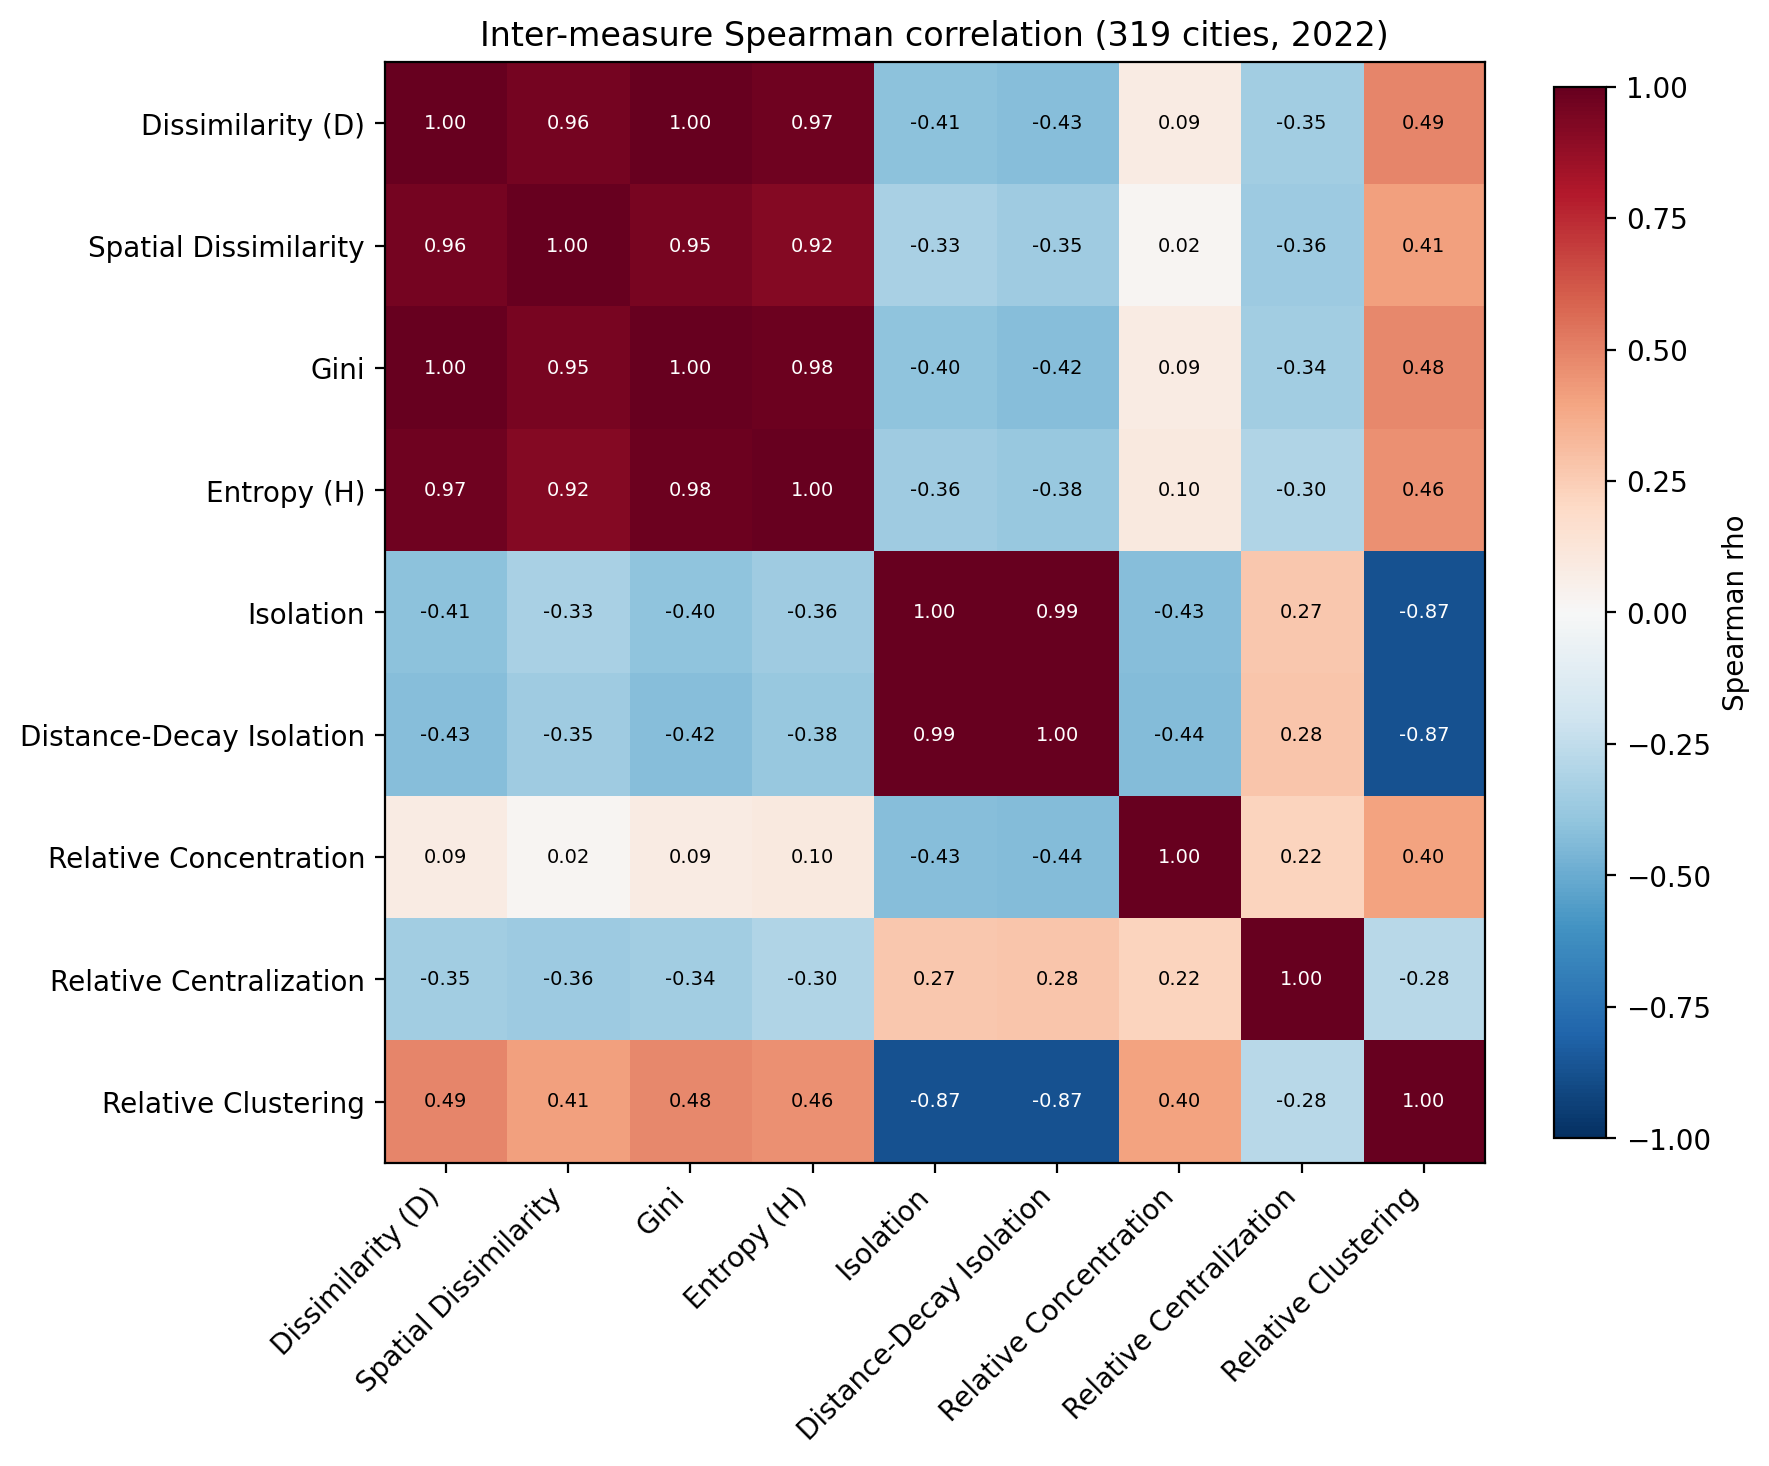
\includegraphics[width=\textwidth]{fig_correlation.png}
\caption{Spearman rank correlation between the nine segregation indices across the 319 cities.}
\label{fig:correlation}
\end{figure}

\begin{figure}[h]
\centering
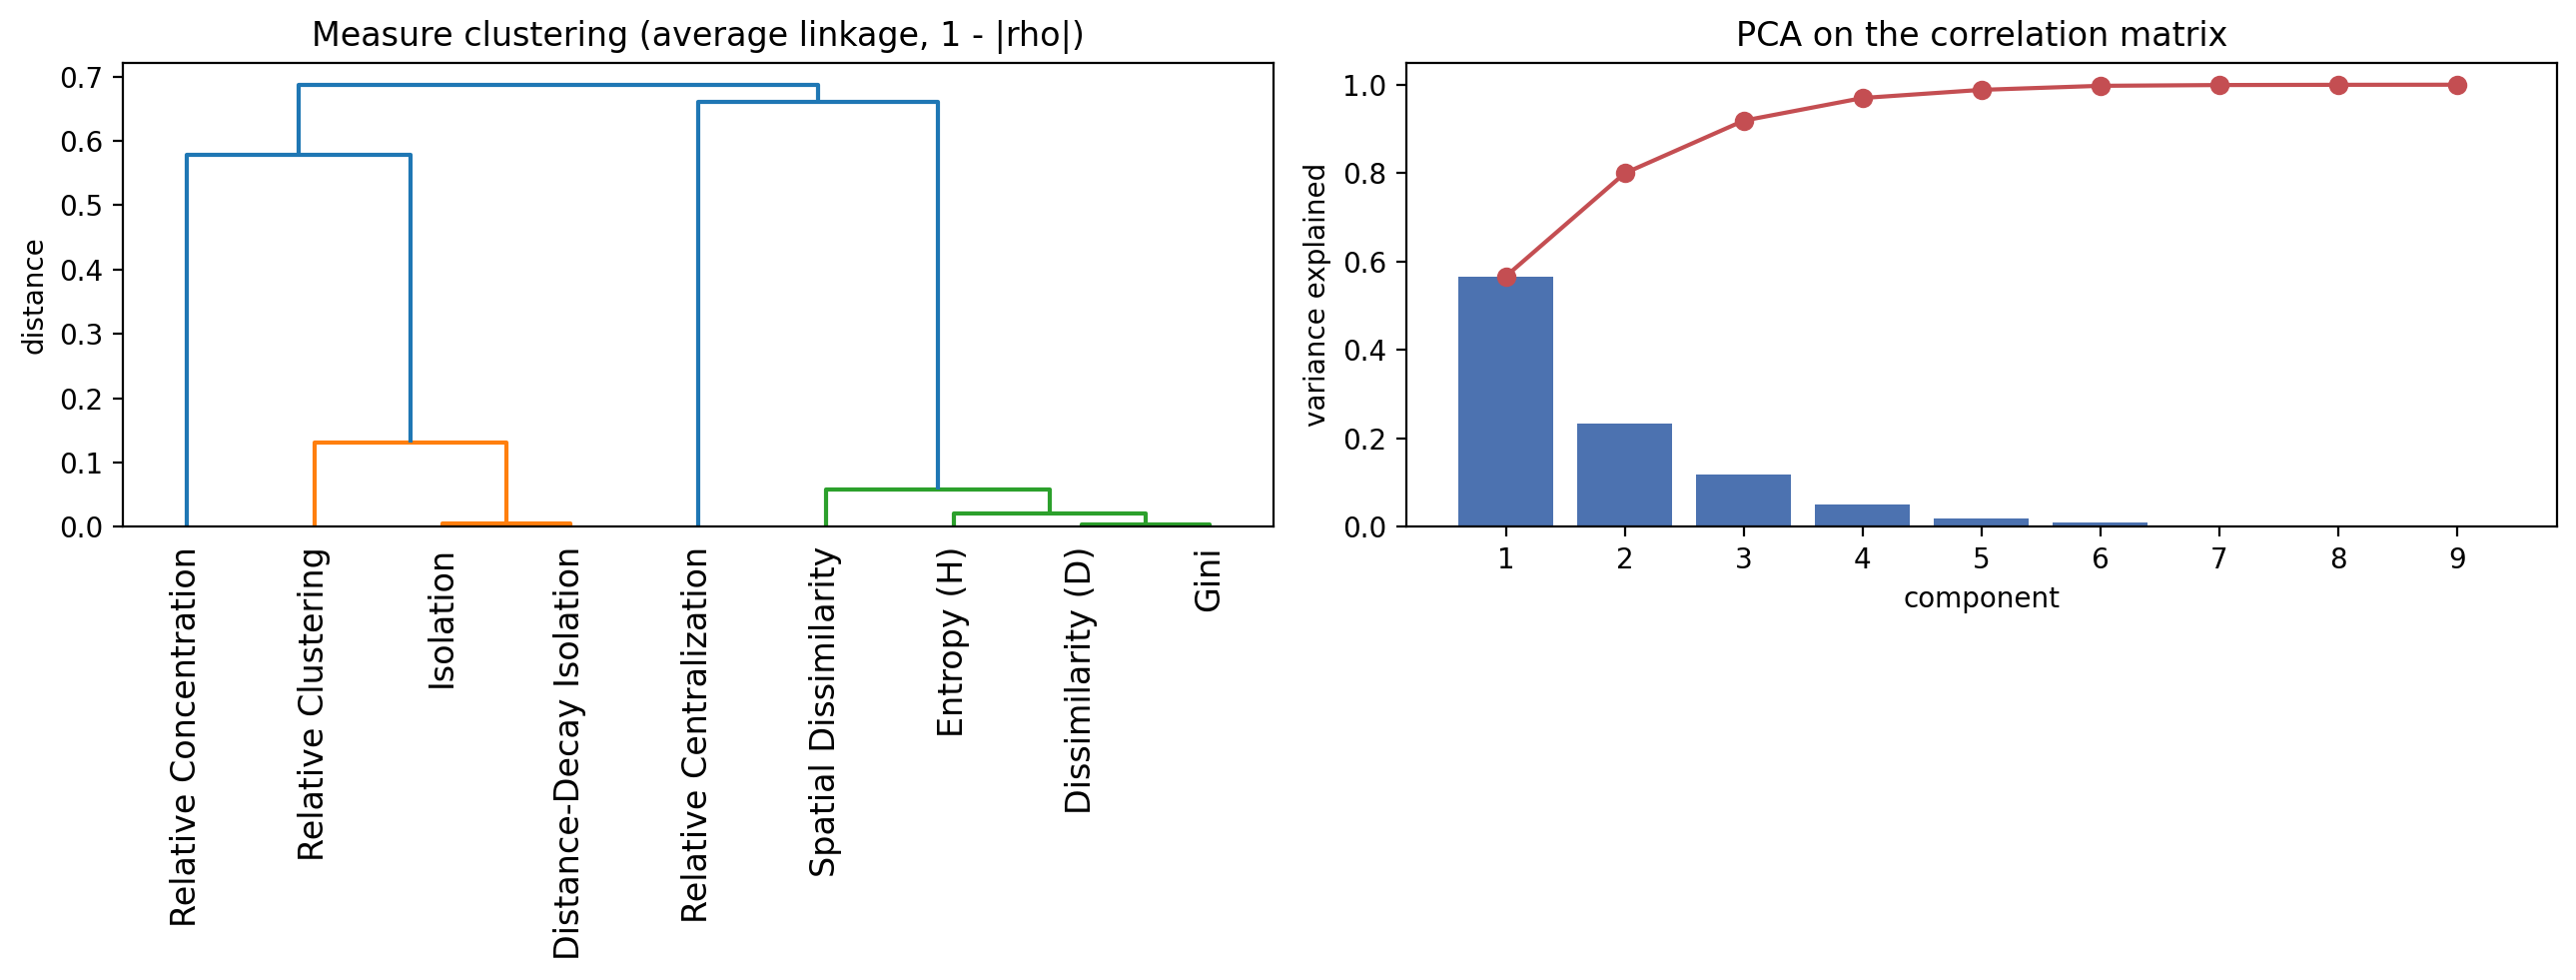
\includegraphics[width=\textwidth]{fig_measure_clustering.png}
\caption{Hierarchical clustering of the nine indices by rank-correlation distance.}
\label{fig:clustering}
\end{figure}

\begin{table}
\caption{Correlação de Spearman entre os nove índices de segregação (nível cidade, Censo 2022). Colunas: D=Dissimilaridade, SD=Dissimilaridade espacial, G=Gini, H=Entropia, Iso=Isolamento, DDI=Isolamento com decaimento, RCo=Concentração relativa, RCe=Centralização relativa, RCl=Agrupamento relativo.}
\label{tab:corr}
\begin{tabular}{lrrrrrrrrr}
\toprule
 & D & SD & G & H & Iso & DDI & RCo & RCe & RCl \\
Medida &  &  &  &  &  &  &  &  &  \\
\midrule
Dissimilarity (D) & 1.00 & 0.96 & 1.00 & 0.97 & -0.41 & -0.43 & 0.09 & -0.35 & 0.49 \\
Spatial Dissimilarity & 0.96 & 1.00 & 0.95 & 0.92 & -0.33 & -0.35 & 0.02 & -0.36 & 0.41 \\
Gini & 1.00 & 0.95 & 1.00 & 0.98 & -0.40 & -0.42 & 0.09 & -0.34 & 0.48 \\
Entropy (H) & 0.97 & 0.92 & 0.98 & 1.00 & -0.36 & -0.38 & 0.10 & -0.30 & 0.46 \\
Isolation & -0.41 & -0.33 & -0.40 & -0.36 & 1.00 & 0.99 & -0.43 & 0.27 & -0.87 \\
Distance-Decay Isolation & -0.43 & -0.35 & -0.42 & -0.38 & 0.99 & 1.00 & -0.44 & 0.28 & -0.87 \\
Relative Concentration & 0.09 & 0.02 & 0.09 & 0.10 & -0.43 & -0.44 & 1.00 & 0.22 & 0.40 \\
Relative Centralization & -0.35 & -0.36 & -0.34 & -0.30 & 0.27 & 0.28 & 0.22 & 1.00 & -0.28 \\
Relative Clustering & 0.49 & 0.41 & 0.48 & 0.46 & -0.87 & -0.87 & 0.40 & -0.28 & 1.00 \\
\bottomrule
\end{tabular}
\end{table}


\subsection{Which cities are most segregated?}\label{sec:rank}

Figure~\ref{fig:rankings} ranks cities on each index and Table~\ref{tab:rankcorr} reports Kendall rank correlations between the rankings. The cities with the highest Dissimilarity are Nova Lima (MG, 0.458), Vit\'oria (ES), Niter\'oi (RJ), Salvador (BA) and Santana de Parna\'iba (SP) --- affluent metropolitan cores and high-income suburbs drawn from several regions. The ranking by Isolation is entirely different: Sim\~oes Filho (BA), Manacapuru (AM), Bragan\c{c}a (PA), Cod\'o (MA) and Salvador (BA) lead, almost all of them in Bahia, Par\'a, Maranh\~ao or Amazonas, where the \emph{preta}$+$\emph{parda} share is locally very high. The ranking by Relative Clustering is different again: Balne\'ario Cambori\'u (SC, 1.012), Santa Cruz do Sul (RS), Porto Alegre (RS) and Florian\'opolis (SC) top the list, almost all of them in Rio Grande do Sul and Santa Catarina. Kendall's $\tau$ between the Dissimilarity and Isolation rankings is $-0.26$, and their top-five lists overlap in at most one city (Salvador). ``The most segregated city in Brazil'' therefore has no answer that does not depend on the dimension chosen.

\begin{figure}[h]
\centering
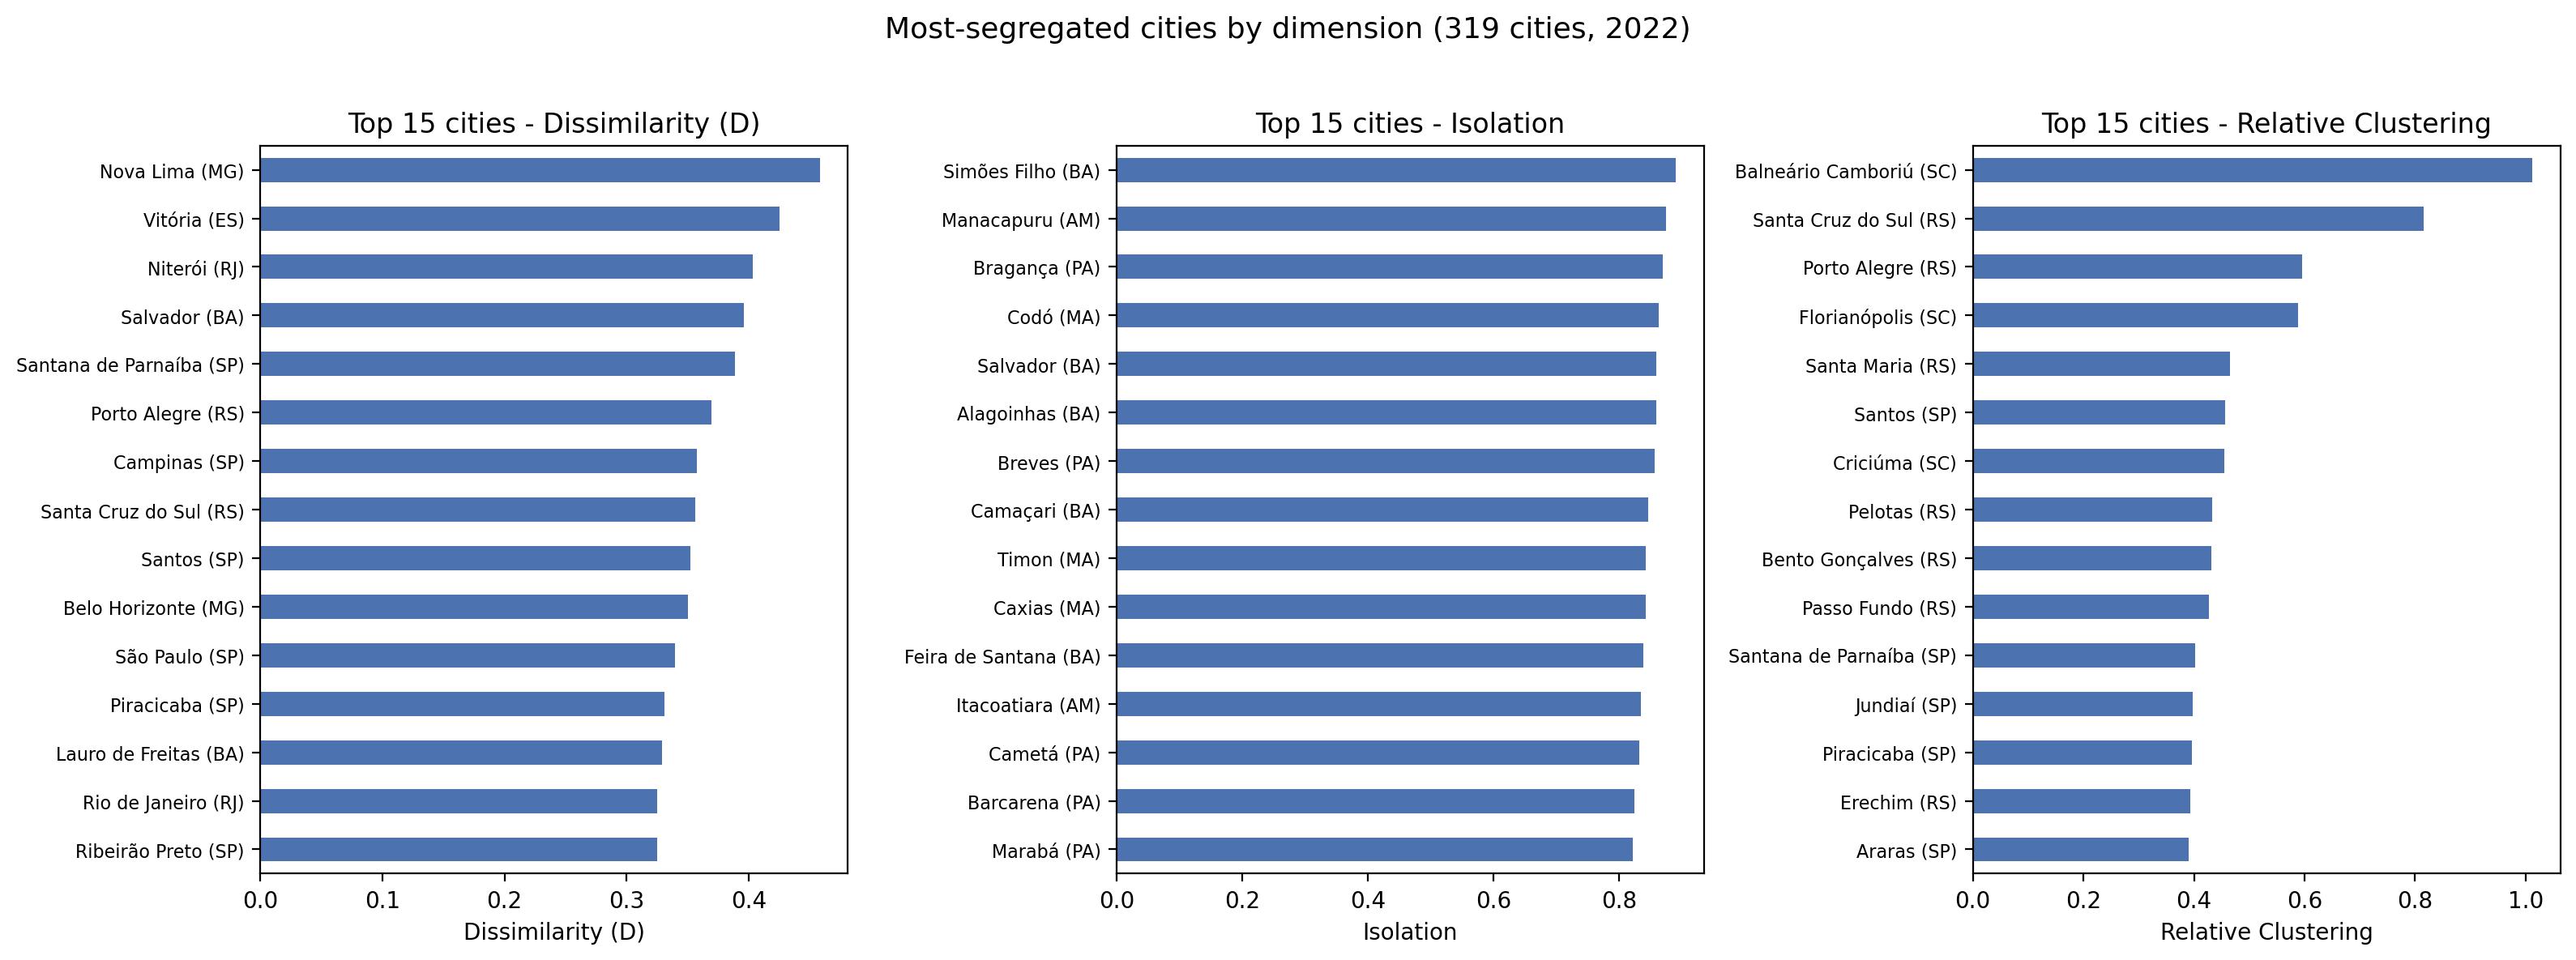
\includegraphics[width=\textwidth]{fig_rankings.png}
\caption{The fifteen highest-scoring cities on three contrasting indices: Dissimilarity, Isolation and Relative Clustering.}
\label{fig:rankings}
\end{figure}

\begin{table}
\caption{Correlação de postos de Kendall (tau) entre os ordenamentos de cidades pelos nove índices de segregação (nível cidade, Censo 2022). Colunas: D=Dissimilaridade, SD=Dissimilaridade espacial, G=Gini, H=Entropia, Iso=Isolamento, DDI=Isolamento com decaimento, RCo=Concentração relativa, RCe=Centralização relativa, RCl=Agrupamento relativo.}
\label{tab:rankcorr}
\begin{tabular}{lrrrrrrrrr}
\toprule
 & D & SD & G & H & Iso & DDI & RCo & RCe & RCl \\
\midrule
Dissimilarity (D) & 1.00 & 0.83 & 0.96 & 0.89 & -0.26 & -0.28 & 0.06 & -0.25 & 0.35 \\
Spatial Dissimilarity & 0.83 & 1.00 & 0.82 & 0.76 & -0.21 & -0.23 & 0.01 & -0.25 & 0.29 \\
Gini & 0.96 & 0.82 & 1.00 & 0.91 & -0.26 & -0.27 & 0.06 & -0.24 & 0.34 \\
Entropy (H) & 0.89 & 0.76 & 0.91 & 1.00 & -0.23 & -0.25 & 0.06 & -0.22 & 0.32 \\
Isolation & -0.26 & -0.21 & -0.26 & -0.23 & 1.00 & 0.94 & -0.30 & 0.18 & -0.67 \\
Distance-Decay Isolation & -0.28 & -0.23 & -0.27 & -0.25 & 0.94 & 1.00 & -0.30 & 0.18 & -0.68 \\
Relative Concentration & 0.06 & 0.01 & 0.06 & 0.06 & -0.30 & -0.30 & 1.00 & 0.15 & 0.27 \\
Relative Centralization & -0.25 & -0.25 & -0.24 & -0.22 & 0.18 & 0.18 & 0.15 & 1.00 & -0.19 \\
Relative Clustering & 0.35 & 0.29 & 0.34 & 0.32 & -0.67 & -0.68 & 0.27 & -0.19 & 1.00 \\
\bottomrule
\end{tabular}
\end{table}


\subsection{Regional patterns}\label{sec:region}

Table~\ref{tab:regional} and Figure~\ref{fig:regional} give the median of each index by macro-region. The evenness measures, Relative Clustering and Relative Concentration all rise broadly from the North and Northeast towards the Southeast and South. Median Dissimilarity moves from 0.176 in the North to 0.219 in the Southeast and 0.217 in the South; median Relative Clustering from $-0.058$ in the North to 0.206 in the South; and median Relative Concentration from $-0.649$ in the North to 0.096 in the South. This pattern confirms and extends the finding of \citet{deSouza2023nationwide_english} --- who reported the South and Southeast as most segregated on Dissimilarity with 2010 data --- to the 2022 Census and to every evenness measure as well as to clustering. The exposure dimension inverts completely. Median Isolation is 0.790 in the North and 0.741 in the Northeast against 0.329 in the South, and Distance-Decay Isolation runs from 0.832 in the North to 0.323 in the South. Relative Centralization varies negligibly across regions, with a spread of about 0.037 between the extreme regional medians. These regional medians are unweighted across cities.

\begin{figure}[h]
\centering

\includegraphics[width=\textwidth]{fig_regional.png}
\caption{Each segregation index by macro-region (box plots), for the 319 cities.}
\label{fig:regional}
\end{figure}

\begin{table}
\caption{Mediana de cada índice de segregação por macrorregião (nível cidade, Censo 2022). Colunas: D=Dissimilaridade, SD=Dissimilaridade espacial, G=Gini, H=Entropia, Iso=Isolamento, DDI=Isolamento com decaimento, RCo=Concentração relativa, RCe=Centralização relativa, RCl=Agrupamento relativo.}
\label{tab:regional}
\begin{tabular}{lrrrrrrrrr}
\toprule
 & D & SD & G & H & Iso & DDI & RCo & RCe & RCl \\
Região &  &  &  &  &  &  &  &  &  \\
\midrule
Norte & 0.176 & 0.108 & 0.256 & 0.041 & 0.790 & 0.832 & -0.649 & -0.061 & -0.058 \\
Nordeste & 0.171 & 0.106 & 0.246 & 0.034 & 0.741 & 0.764 & -0.303 & -0.045 & -0.065 \\
Centro-Oeste & 0.177 & 0.098 & 0.252 & 0.037 & 0.644 & 0.682 & -0.144 & -0.068 & 0.015 \\
Sudeste & 0.219 & 0.128 & 0.306 & 0.055 & 0.537 & 0.529 & -0.063 & -0.082 & 0.093 \\
Sul & 0.217 & 0.136 & 0.299 & 0.051 & 0.329 & 0.323 & 0.096 & -0.069 & 0.206 \\
\bottomrule
\end{tabular}
\end{table}


\subsection{Minority share and segregation}\label{sec:share}

Figure~\ref{fig:minorityshare} plots each index against the city-wide \emph{preta}$+$\emph{parda} share, together with a LOESS smoother. Isolation and Distance-Decay Isolation increase almost linearly with the minority share, the points hugging the diagonal. This is close to an arithmetic identity: when a group is spread evenly, its isolation index approaches its population share, so a rising curve here is not evidence of stronger spatial sorting in cities where the minority is larger. The evenness measures show a weak negative relationship with the minority share. Relative Clustering declines more steeply as the share grows, and Relative Concentration shows a moderate negative pattern that steepens at the highest shares. Relative Centralization is essentially flat across the range. No test is carried out; the description refers only to the scatter and its smoother.

\begin{figure}[h]
\centering

\includegraphics[width=\textwidth]{fig_minorityshare.png}
\caption{Each segregation index against the city-wide \emph{preta}$+$\emph{parda} population share, with a LOESS smoother.}
\label{fig:minorityshare}
\end{figure}

\subsection{The spatial texture of segregation}\label{sec:maps}

Figure~\ref{fig:maps-national} maps the 319 cities as one dot each, coloured by Dissimilarity and by Spatial Dissimilarity, over a light state-boundary layer. The higher-scoring cities form a visible cluster in the Southeast and South, while the North, Northeast and Centre-West appear consistently paler; the two panels tell the same story. Figure~\ref{fig:maps-cities} shows tract-level maps of the \emph{preta}$+$\emph{parda} share for six large cities --- Porto Alegre, S\~ao Paulo, Rio de Janeiro, Belo Horizonte, Florian\'opolis and Recife. Each displays the classic centre--periphery gradient: pale, low-minority-share areas in the affluent urban core and darker areas towards the periphery. S\~ao Paulo and Recife are the clearest instances of this arrangement. Together the two sets of maps make concrete the numerical patterns of the preceding subsections: the regional concentration of evenness in the South and Southeast, and, within individual cities, the core--periphery structure that underlies the city-level indices.

\begin{figure}[h]
\centering
\begin{subfigure}[b]{0.48\textwidth}
\centering
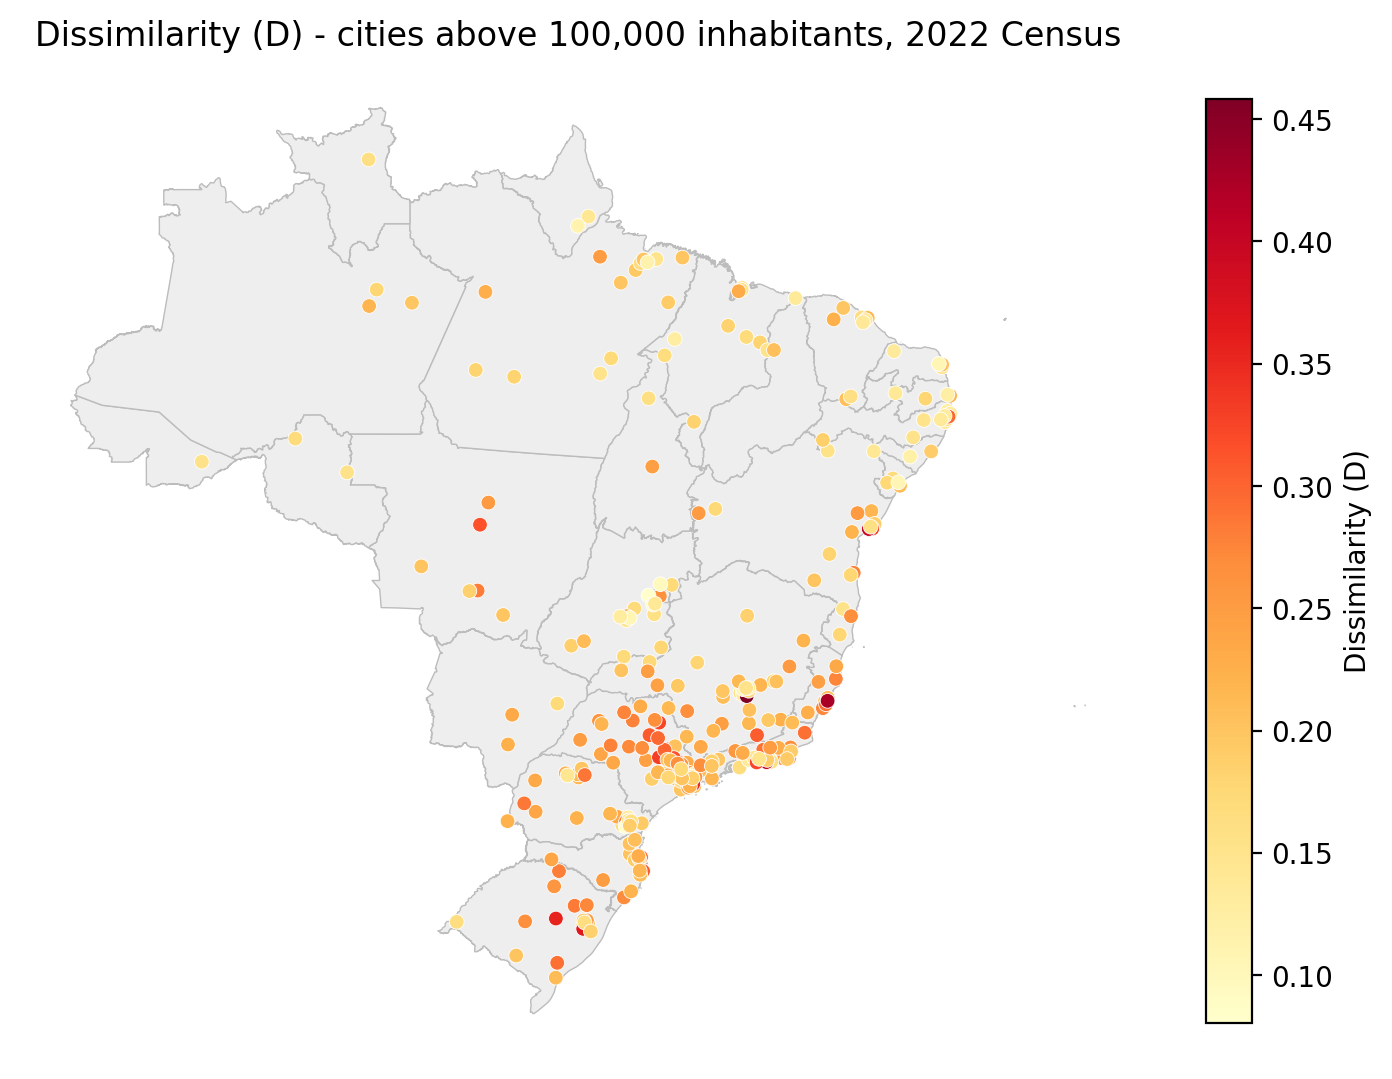
\includegraphics[width=\textwidth]{fig_map_national_dissim.png}
\caption{Dissimilarity index}
\label{fig:map-dissim}
\end{subfigure}
\hfill
\begin{subfigure}[b]{0.48\textwidth}
\centering
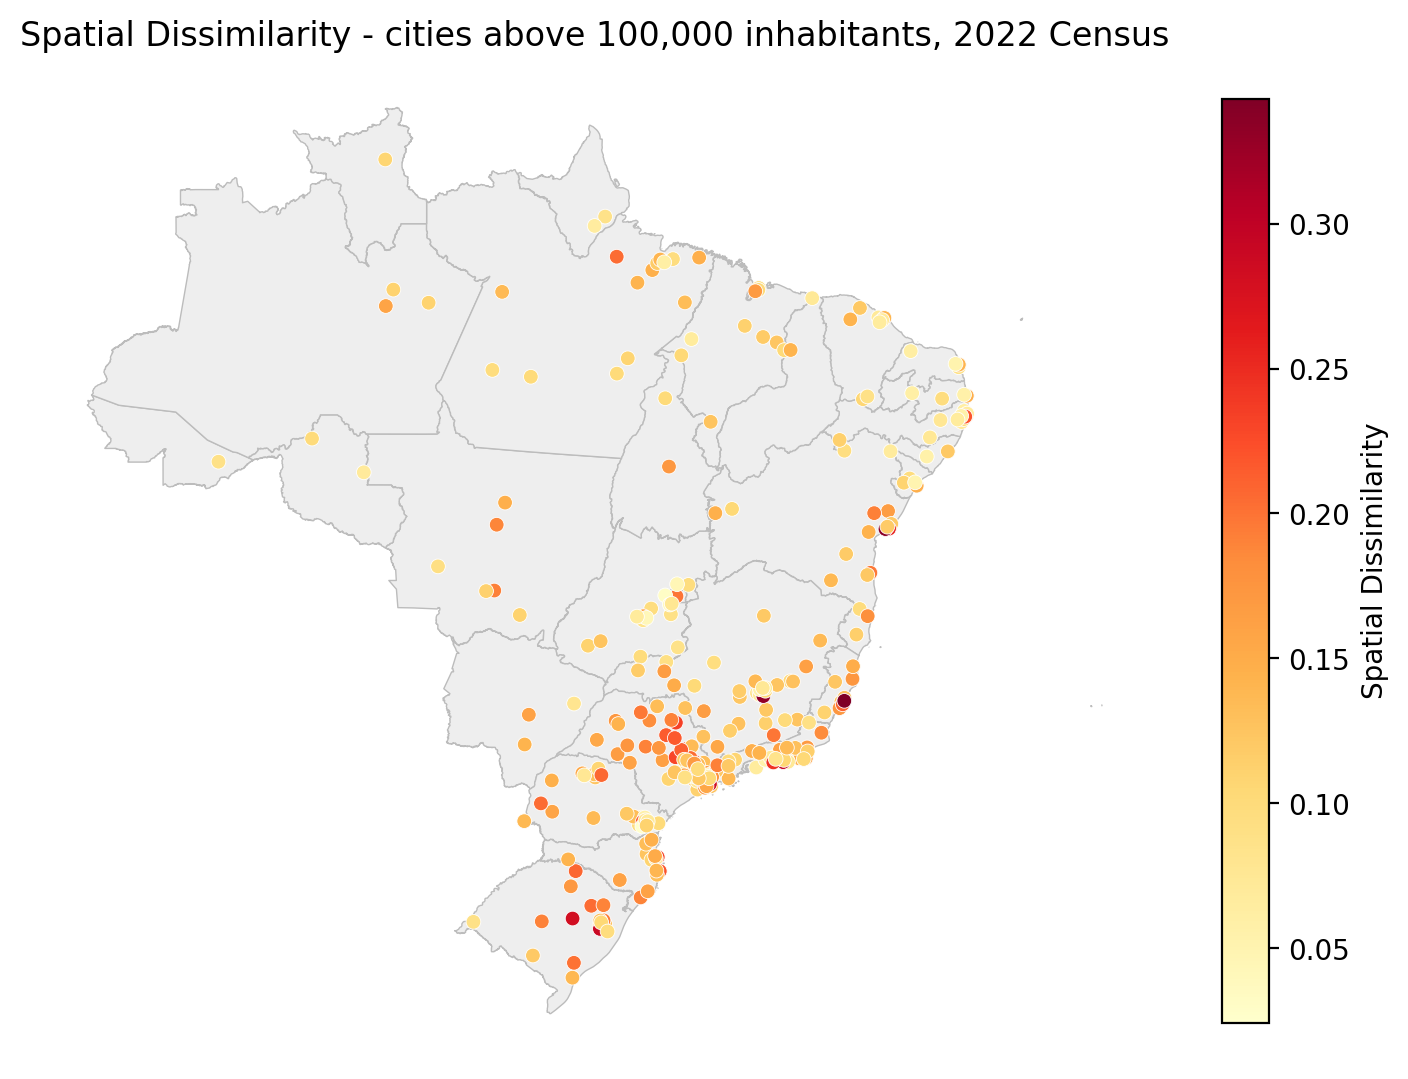
\includegraphics[width=\textwidth]{fig_map_national_spatial.png}
\caption{Spatial Dissimilarity index}
\label{fig:map-spatial}
\end{subfigure}
\caption{Racial residential segregation across the 319 municipalities: one point per city, over state boundaries.}
\label{fig:maps-national}
\end{figure}

\begin{figure}[h]
\centering
\begin{subfigure}[b]{0.32\textwidth}
\centering
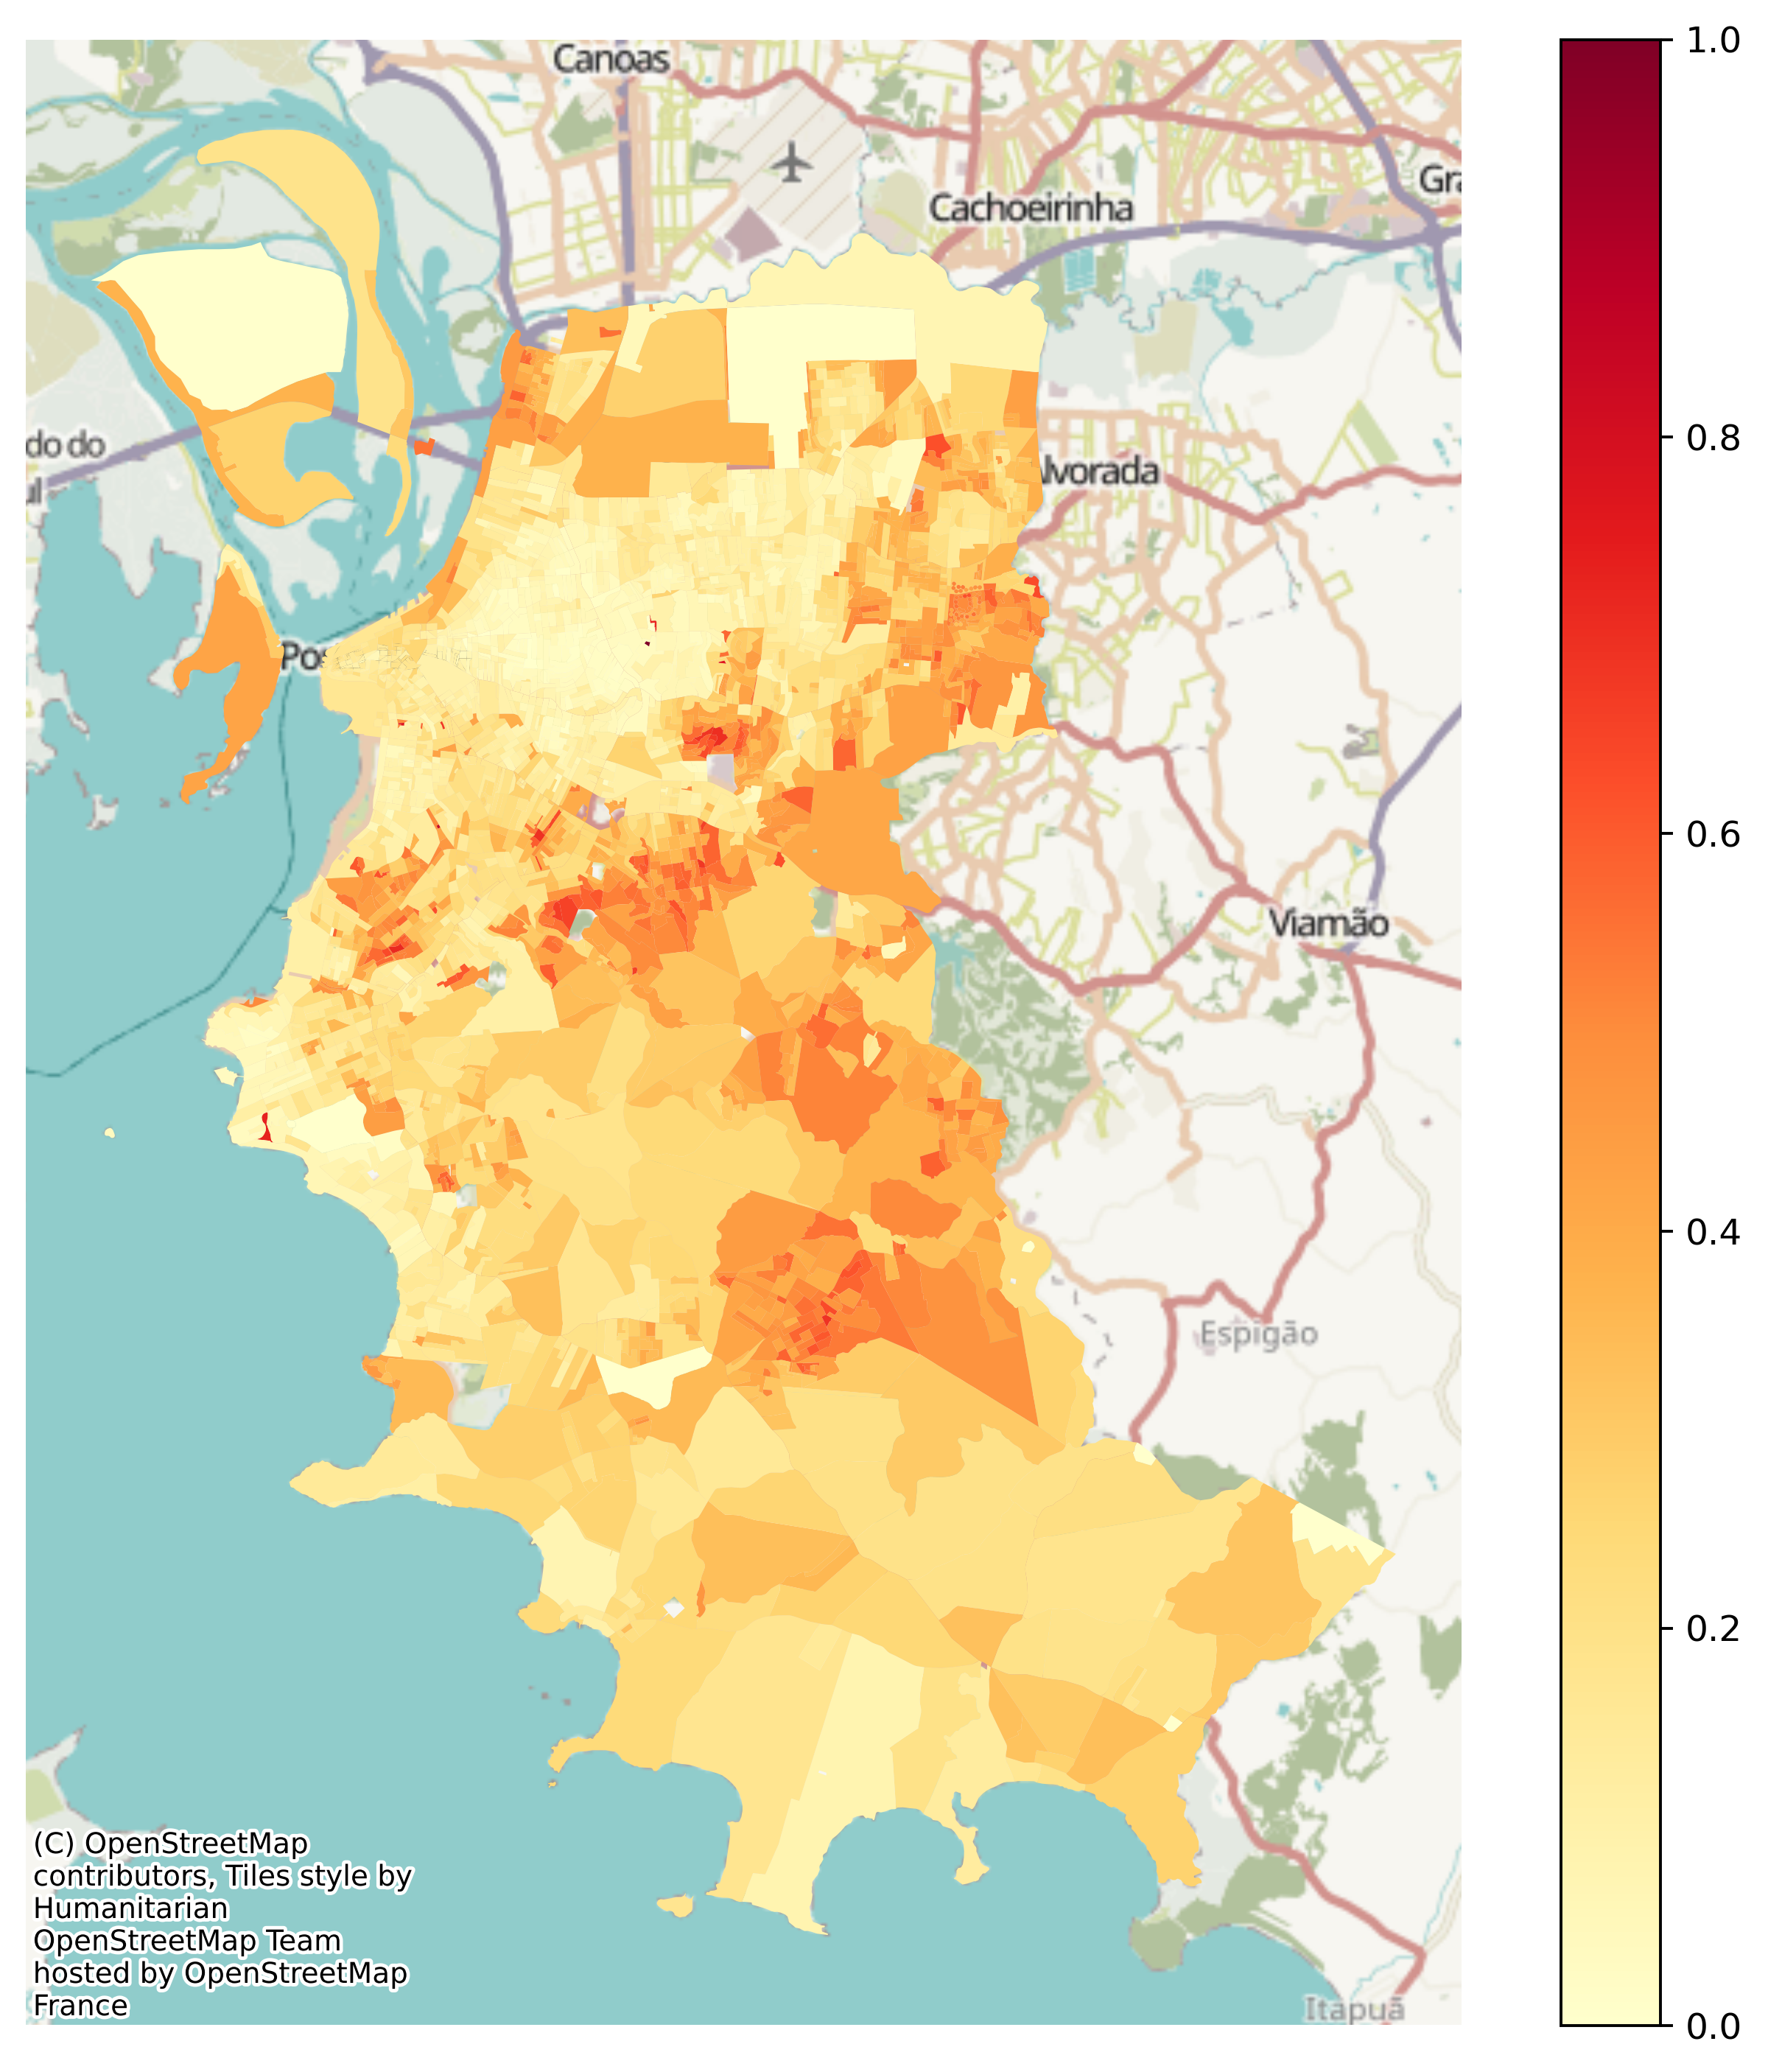
\includegraphics[width=\textwidth]{seg_profile_4314902.png}
\caption{Porto Alegre}
\label{fig:city-pa}
\end{subfigure}
\hfill
\begin{subfigure}[b]{0.32\textwidth}
\centering
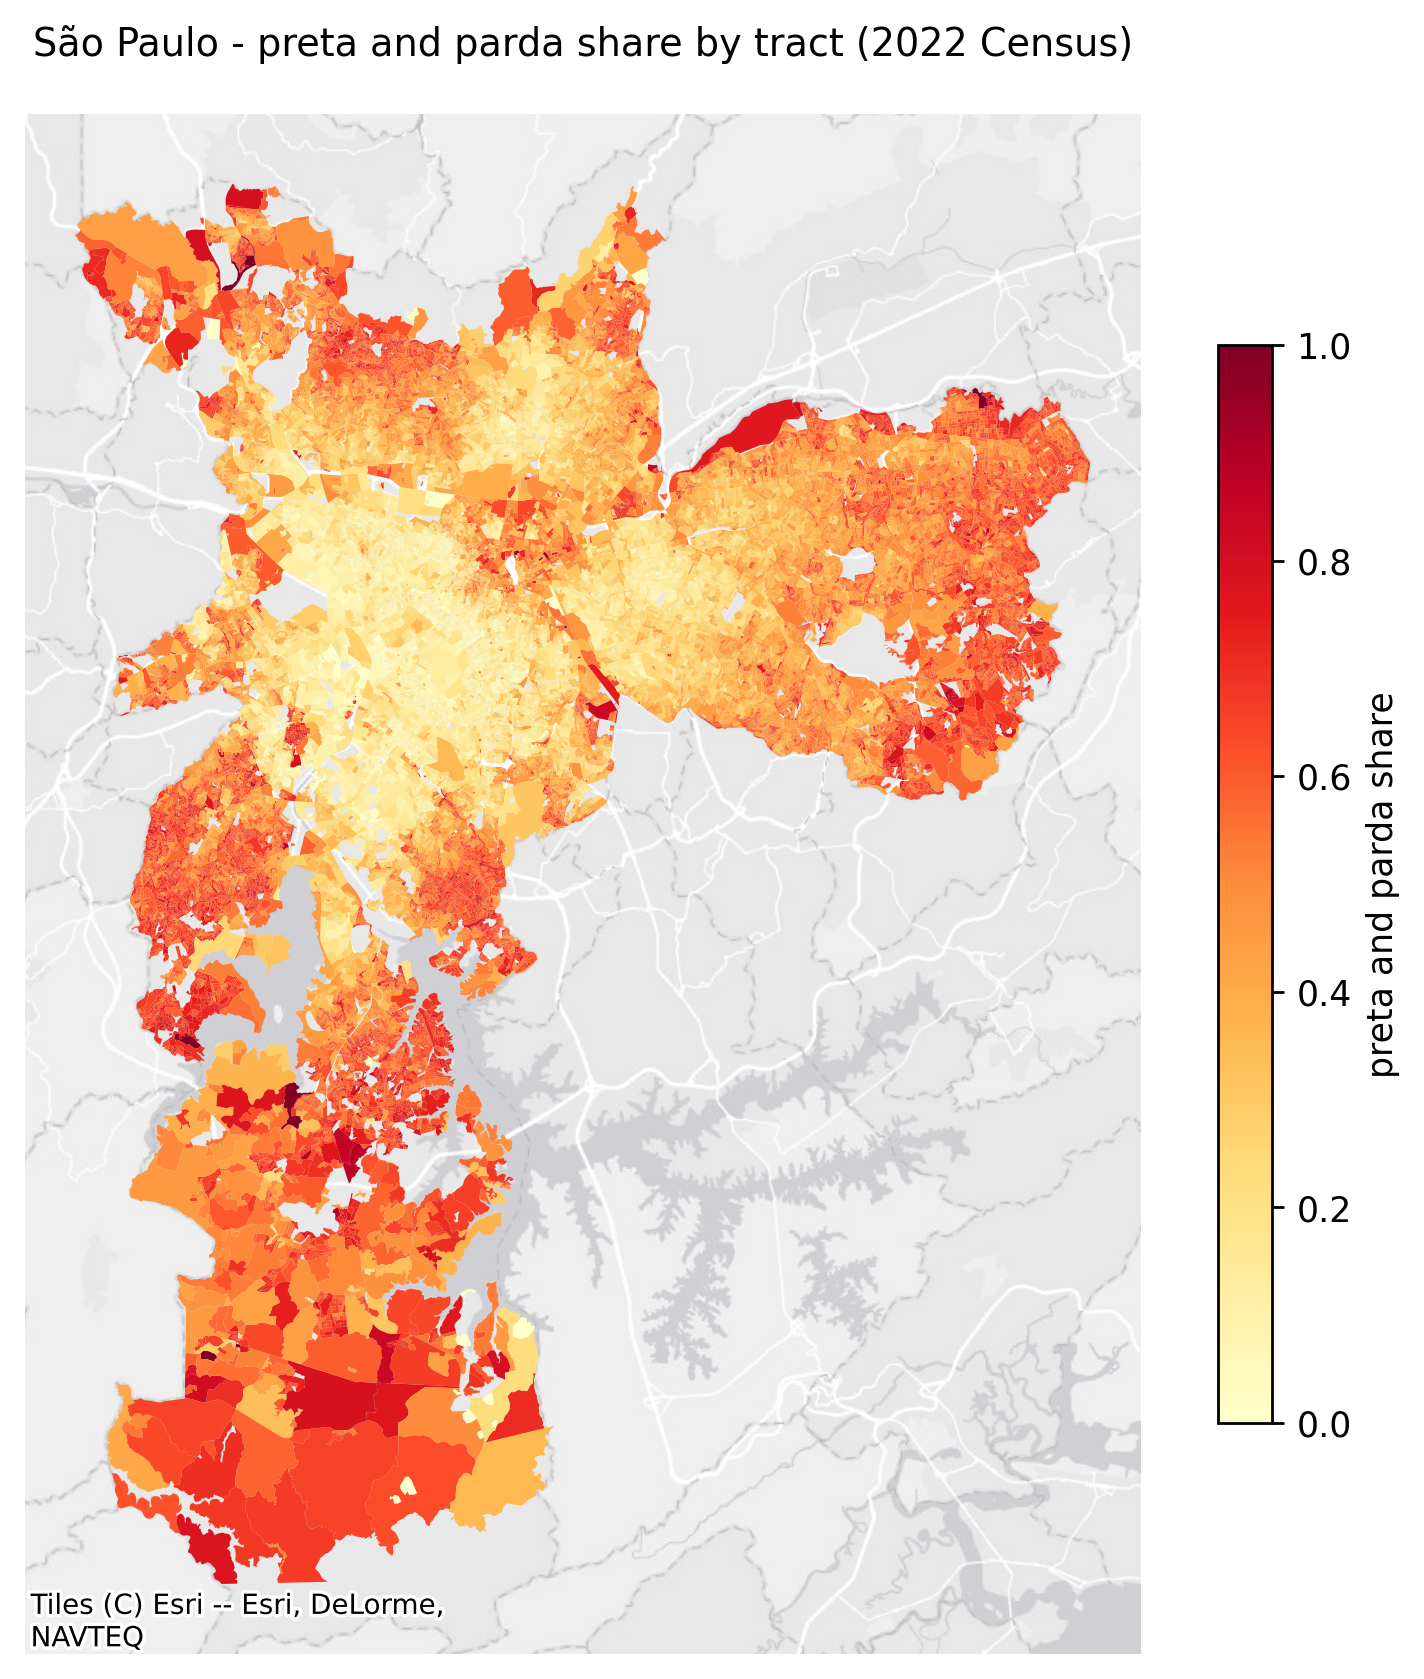
\includegraphics[width=\textwidth]{seg_profile_3550308.png}
\caption{São Paulo}
\label{fig:city-sp}
\end{subfigure}
\hfill
\begin{subfigure}[b]{0.32\textwidth}
\centering
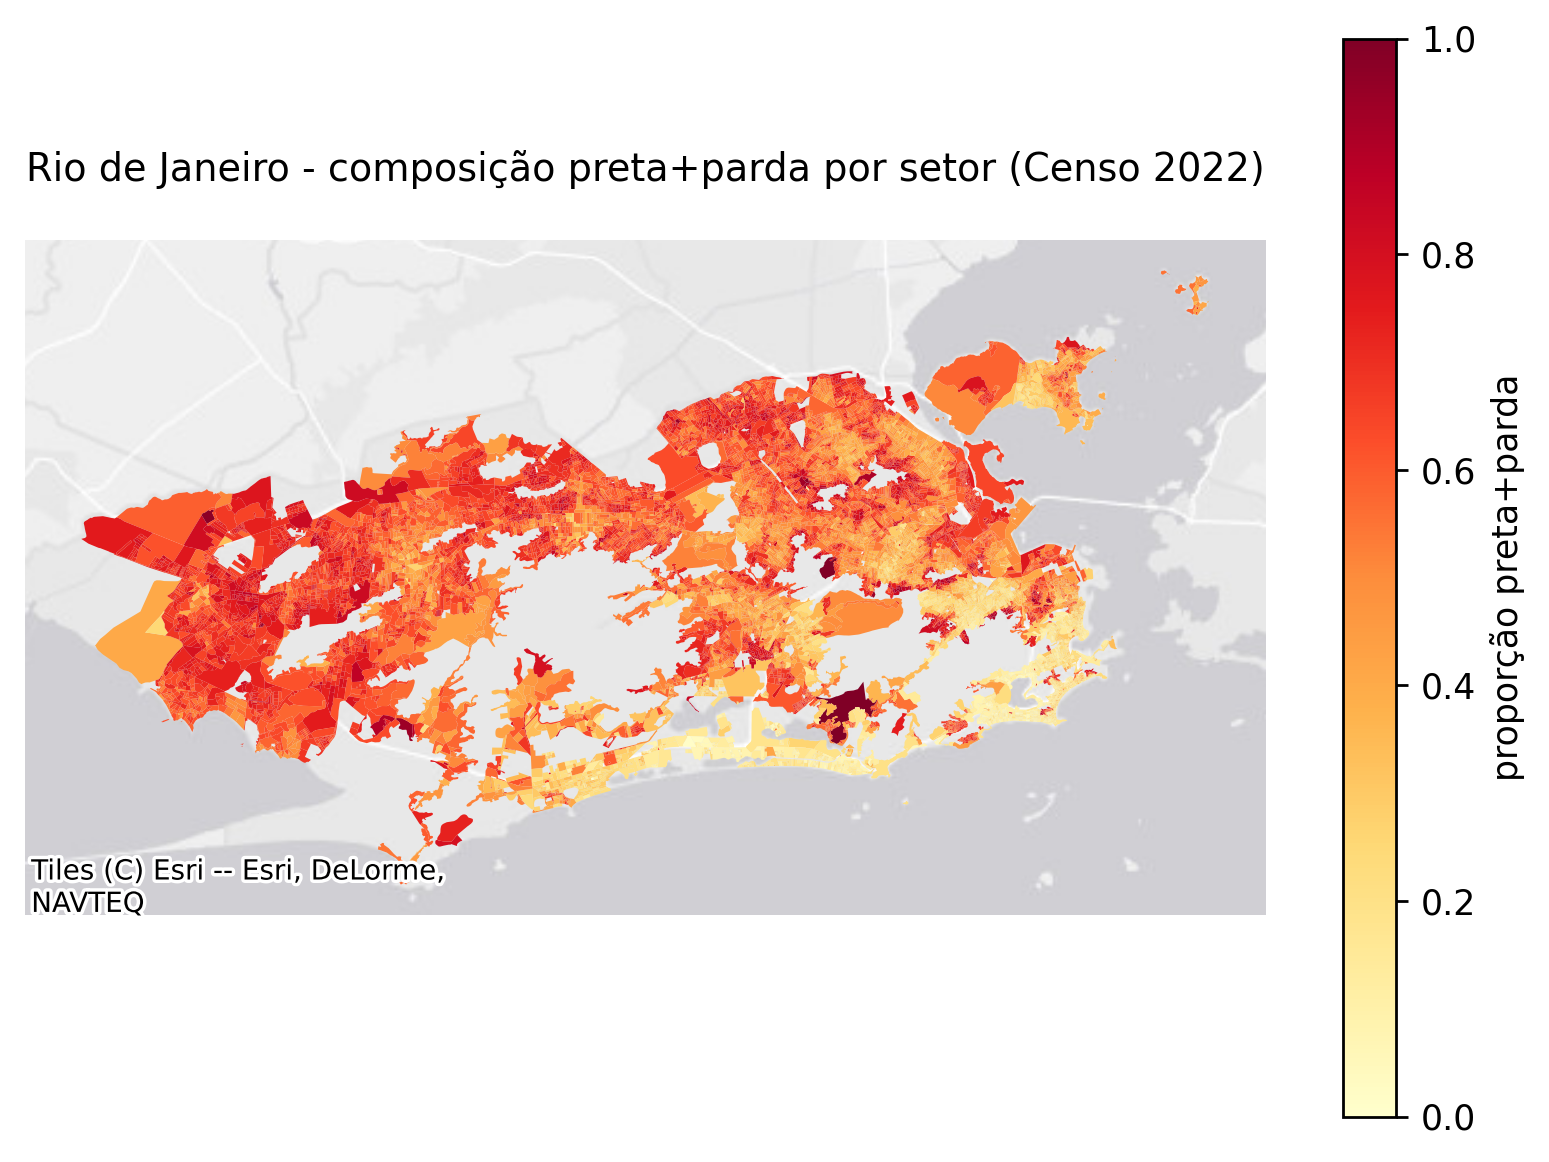
\includegraphics[width=\textwidth]{seg_profile_3304557.png}
\caption{Rio de Janeiro}
\label{fig:city-rj}
\end{subfigure}

\begin{subfigure}[b]{0.32\textwidth}
\centering
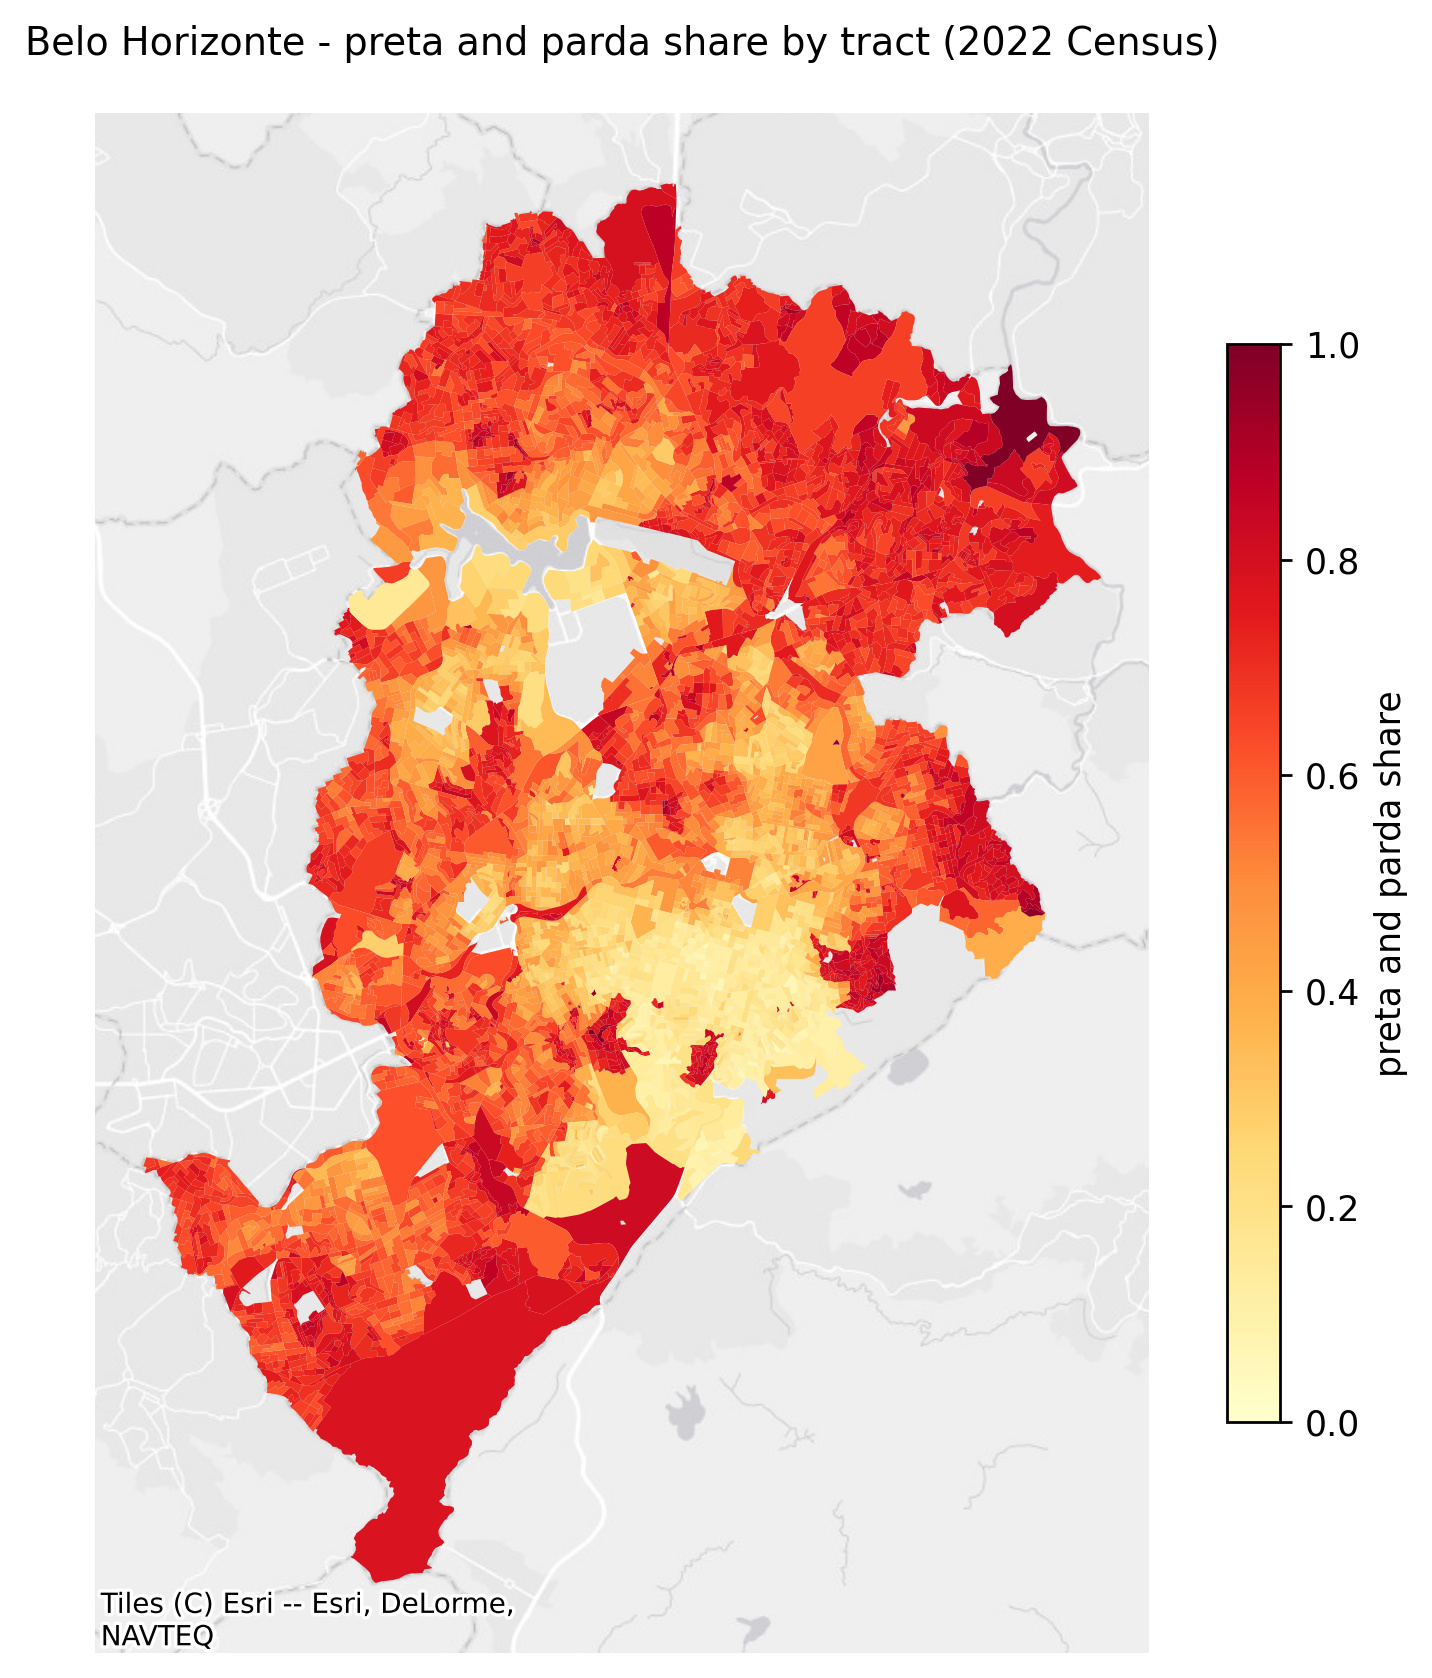
\includegraphics[width=\textwidth]{seg_profile_3106200.png}
\caption{Belo Horizonte}
\label{fig:city-bh}
\end{subfigure}
\hfill
\begin{subfigure}[b]{0.32\textwidth}
\centering
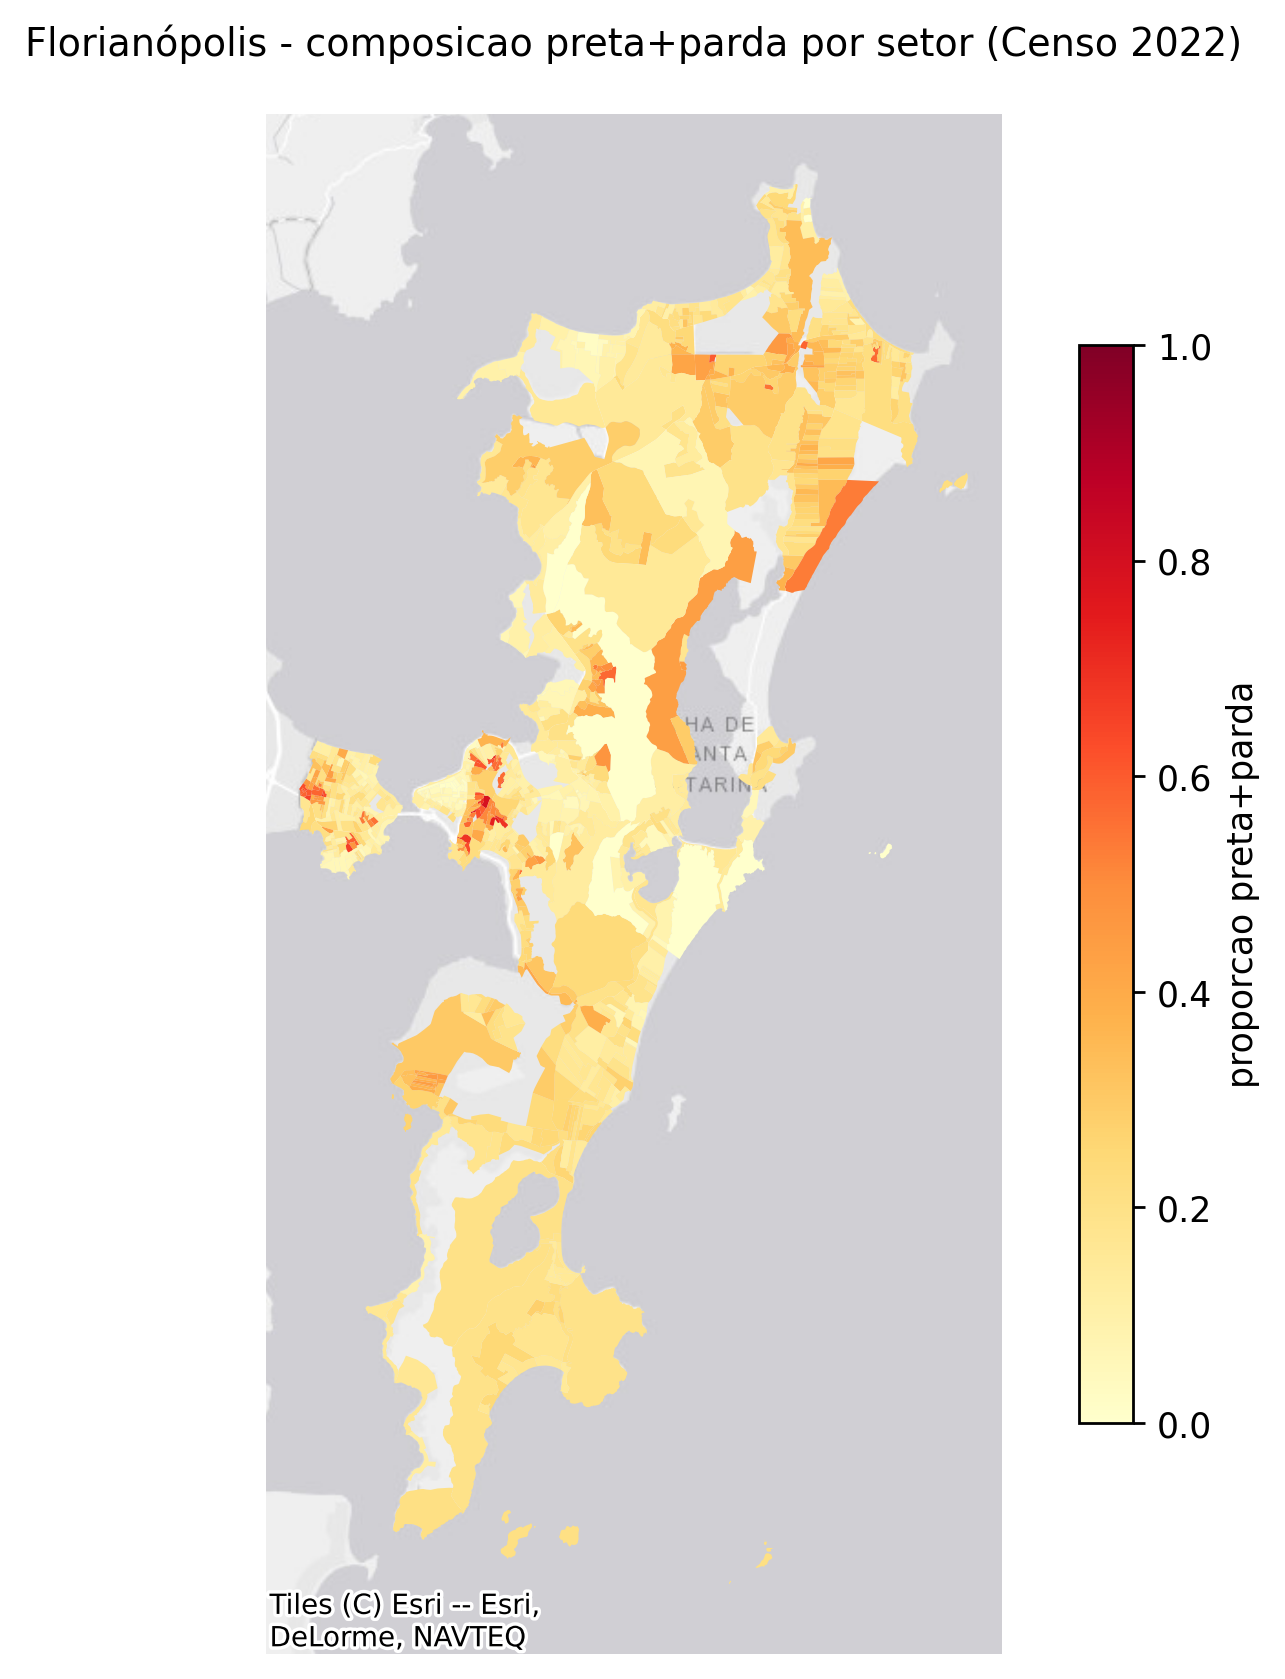
\includegraphics[width=\textwidth]{seg_profile_4205407.png}
\caption{Florianópolis}
\label{fig:city-fl}
\end{subfigure}
\hfill
\begin{subfigure}[b]{0.32\textwidth}
\centering
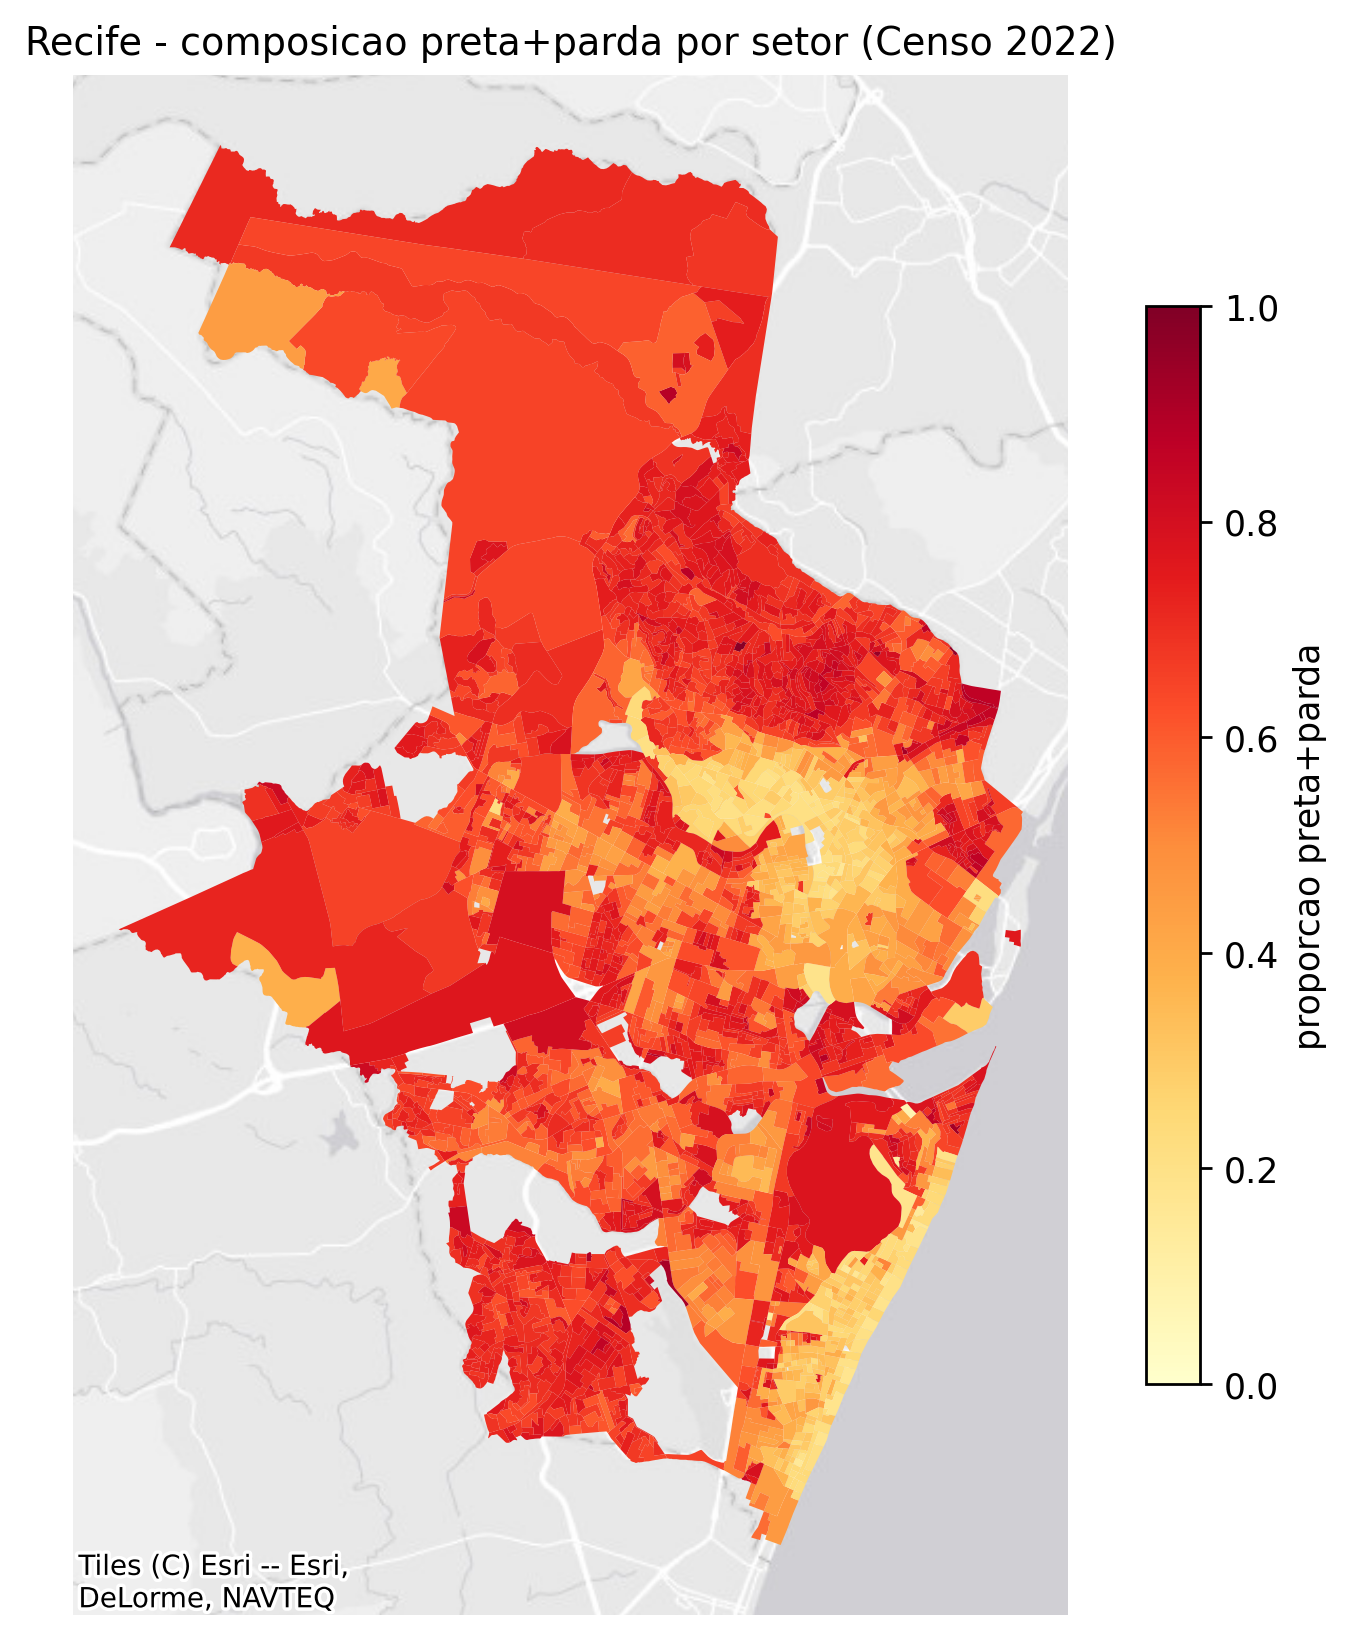
\includegraphics[width=\textwidth]{seg_profile_2611606.png}
\caption{Recife}
\label{fig:city-rc}
\end{subfigure}

\caption{Tract-level \emph{preta}$+$\emph{parda} population share for six large cities.}
\label{fig:maps-cities}
\end{figure}

\section{Discussion}\label{sec:discussion}

The four evenness indices are near-redundant across the Brazilian urban system (Section~\ref{sec:agree}): their pairwise rank correlations never fall below 0.92, and Dissimilarity and Gini are for practical purposes the same statistic. On this evidence the Brazilian literature's near-exclusive reliance on $D$ has cost little information \emph{within} the evenness dimension --- a spatially explicit or entropy-based evenness measure would have ordered the cities almost identically. What that reliance has done is leave the other four dimensions unobserved, and those dimensions are not redundant with evenness. The exposure dimension produces the opposite regional ranking to evenness (Section~\ref{sec:region}), and the identity of ``the most segregated city'' changes completely with the dimension chosen: the leading cities on Dissimilarity and on Isolation overlap in at most one case, and the two rankings correlate negatively (Section~\ref{sec:rank}). Concentration and centralization, in turn, vary almost independently of the rest (Section~\ref{sec:agree}). A one-index characterisation of Brazilian racial segregation is therefore incomplete, and for the exposure dimension it is potentially misleading, because $D$ and Isolation move in opposite directions across the country.

The divergence between exposure and evenness is compositional in origin. The isolation index is bounded below by the group's population share: where \emph{preta}$+$\emph{parda} residents form a large local majority --- as they do across much of the North and Northeast, with regional median shares near 0.75 --- a member's expected own-group neighbourhood share is high almost by construction, whatever the spatial arrangement of the tracts (Section~\ref{sec:share}). High isolation in those regions thus coincides with unremarkable evenness. Evenness and clustering pick out a different geography: the consolidated, high-income metropolitan cores of the Southeast and South, where the population is spatially sorted and where a gated-enclave, fragmented urbanism has been documented in detail \citep{barros2024saopaulolondres, danilofranca2022fortaleza, telles2004race}. The centre--periphery gradient visible in the city maps --- pale, low-minority-share affluent cores against darker peripheries, clearest in S\~ao Paulo and Recife (Section~\ref{sec:maps}) --- is the mechanism that generates the evenness and clustering results. The two families of measures are not in tension: they describe different features of the same urban system, one driven by how many minority residents a city has and the other by where those residents live.

On the evenness dimension the results align with and update \citet{deSouza2023nationwide_english}. The South and Southeast remain the most segregated regions in 2022, and this now holds across all four evenness indices and the clustering measure rather than resting on $D$ alone. The contribution beyond confirmation is twofold. First, the exposure dimension inverts the regional ordering, so that the regions with the lowest evenness segregation record the highest isolation. Second, the concentration and centralization dimensions are close to orthogonal to evenness and to each other, so the Brazilian urban system varies along at least two and arguably three independent axes. Neither feature is visible in a design built on the dissimilarity index alone.

Several limitations qualify these results. First, $D$ and its spatial analogue are biased upward when tracts are small, and cities differ in census granularity; we apply no correction \citep{cortese1976further, carrington1997measuring, allen2015more}. Second, the modifiable areal unit problem applies, and IBGE tract boundaries changed between 2010 and 2022, so these values are not directly comparable to the 2010 figures of \citet{deSouza2023nationwide_english} --- the comparable objects are the regional orderings, not the levels. Third, the analysis is cross-sectional, covering 2022 only. Fourth, the \emph{preta}$+$\emph{parda} aggregation masks distinctions between the \emph{preto} and \emph{pardo} populations. Fifth, Relative Concentration is unreliable where the minority is the local majority: it collapses toward its lower bound near $-2$ for nine cities with minority share between 0.70 and 0.87, nearly all in the North and Northeast, and its rank correlation with minority share is about $-0.42$; the concentration dimension should be read cautiously for those cities. Sixth, Relative Concentration and Relative Centralization are also sensitive to the areal-unit and urban-core definitions, for which PySAL defaults were used throughout. Seventh, about 1.8\% of tracts carry no census race data and are excluded.

Four extensions follow directly. Simulation-based inference would attach uncertainty to individual values and to comparisons between cities. A spatial-versus-compositional decomposition would separate how much of each between-city difference is locational rather than demographic \citep{rey2021comparative}. A harmonised tract base would allow genuine measurement of change between 2010 and 2022. And street-network-based measures would replace Euclidean distance with travelled distance.

\section{Reproducibility}\label{sec:repro}

The complete pipeline is public. The \texttt{segbr} Python package performs data loading, city assembly and the computation of the nine measures; driver scripts build the city universe and run the nationwide computation; and further scripts generate every figure and table. A pinned environment specification, a manifest of the IBGE source files (\texttt{MANIFEST.md}) and a documented run order accompany the code. Every figure and table in this paper regenerates from the committed city-level results table with a single command, so the analysis can be reproduced end to end or inspected at any intermediate stage. The repository is available at \url{REPOSITORY-URL}.

\section{Conclusion}\label{sec:conclusion}

Racial residential segregation in Brazil is moderate on the evenness dimension, with a median dissimilarity index of about 0.20, and on that dimension it is concentrated in the cities of the South and Southeast --- a picture that the 2022 Census confirms and broadens relative to earlier nationwide work. Evenness, however, is only one of the five dimensions, and the others do not track it. The exposure dimension is highest exactly where evenness is lowest, driven by demographic composition rather than by spatial sorting; clustering singles out the cities of the South; and concentration and centralization vary almost independently of the rest. Characterising Brazilian racial segregation through the dissimilarity index alone is therefore insufficient. A multidimensional, spatially explicit, and --- in future work --- inferential approach is needed to describe how Brazilian cities are actually divided.

%% Funding, author contributions (CRediT), acknowledgements and conflict-of-interest
%% declarations are NOT placed in the manuscript body for REBEP: they go in the
%% "Formulario com informacoes complementares da submissao". See SUBMISSION.md.

\bibliographystyle{plainnat}   % author-date; REBEP wants ABNT NBR 6023 -- see SUBMISSION.md "still to do"
\bibliography{references}

\end{document}
